\documentclass[12pt]{ucthesis}

\usepackage{etex}
\usepackage[morefloats=125]{morefloats}
\usepackage[hyphens]{url}
\usepackage[caption=false]{subfig}
\usepackage{graphicx}
\usepackage{tabularx}
\usepackage{amssymb}
\usepackage{amsmath}
\usepackage{amsthm}
\usepackage[letterpaper]{geometry}
\usepackage[overload]{textcase}
\usepackage{color}
\usepackage[nonumberlist,toc]{glossaries}
\usepackage{wrapfig}
\usepackage{longtable}
\usepackage{morefloats}
\usepackage{float}
\usepackage{listings}
\usepackage{makecell}
\usepackage{appendix}
\usepackage[]{algorithm2e}
\usepackage{titlesec}
\usepackage[breaklinks=true,hidelinks,pdfusetitle]{hyperref}
\usepackage{cleveref}
\usepackage{ifthen}
\usepackage{ulem}

\newcommand{\N}{\mathbb{N}}
\newcommand{\Z}{\mathbb{Z}}
\newcommand{\Q}{\mathbb{Q}}
\newcommand{\R}{\mathbb{R}}
\newcommand{\C}{\mathbb{C}}
\newcommand{\E}{\mathbb{E}}
\newcommand{\e}{\epsilon}
\renewcommand\labelitemi{-}
\newtheorem{theorem}{Theorem}
\newtheorem{lemma}[theorem]{Lemma}
\newtheorem{proposition}[theorem]{Proposition}
\newtheorem{corollary}[theorem]{Corollary}
\theoremstyle{definition}
\newtheorem{definition}[theorem]{Definition}
\newtheorem{example}[theorem]{Example}

\setcounter{secnumdepth}{3}
\setcounter{tocdepth}{3}

% Added to avoid windows and orphans
\usepackage[all]{nowidow}
% Added to fix spacing between footnote entries
\usepackage{setspace}
\newlength{\myfootnotesep}
\setlength{\myfootnotesep}{\baselineskip}
\addtolength{\myfootnotesep}{-\footnotesep}
\setlength{\footnotesep}{\myfootnotesep} % set spacing between footnotes

\makeindex
\makeglossaries

% Shrink the size of headers
\titleformat{\chapter}[display]
        {\normalfont\normalsize\centering}
        {\ifthenelse{\equal{\thechapter}{A}}{APPENDICES\\[4.3ex]}{}\chaptertitlename\ \thechapter}
        {0pt}{\normalsize\uppercase}
\titlespacing*{\chapter}{0pt}{-20pt}{4.3ex plus .2ex}


\titleformat*{\section}{\normalsize\bfseries}
\titleformat*{\subsection}{\small\bfseries}
\titleformat*{\subsubsection}{\small\bfseries}
\titleformat*{\paragraph}{\small\bfseries}
\titleformat*{\subparagraph}{\small\bfseries}

\bibliographystyle{abbrv}

% Make \tindent indent pages if you have no paragraph indent
\newlength\tindent
\setlength{\tindent}{\parindent}
\setlength{\parindent}{0.in} \setlength{\parskip}{1.em}
\renewcommand{\indent}{\hspace*{\tindent}}
% Otherwise, comment out the above and uncomment this for default indentation on each paragraph
%\setlength{\parindent}{0.25in} \setlength{\parskip}{6pt}

\geometry{verbose,nohead,tmargin=1in,bmargin=1in,lmargin=1.5in,rmargin=1in}

% Different font in captions (single-spaced, bold) ------------
\newcommand{\captionfonts}{\small\bf\ssp}

\newcommand{\mycaption}[2]{\caption[#1 --- #2]{#1 --- #2}}

\makeatletter  % Allow the use of @ in command names
\long\def\@makecaption#1#2{%
  \vskip\abovecaptionskip
  \sbox\@tempboxa{{\captionfonts #1: #2}}%
  \ifdim \wd\@tempboxa >\hsize
    {\captionfonts #1: #2\par}
  \else
    \hbox to\hsize{\hfil\box\@tempboxa\hfil}%
  \fi
  \vskip\belowcaptionskip}
\makeatother   % Cancel the effect of \makeatletter
% ---------------------------------------

% Define Appendix refs
\crefname{app}{appendix}{appendices}
\Crefname{app}{Appendix}{Appendices}

% Add Figures folder to the graphics path
\graphicspath{{Figures/}{figures/}}

% Options for hyperref
\hypersetup{
    bookmarksnumbered=true,
    bookmarksopen=false,
    bookmarksopenlevel=0,
    colorlinks=false,
    pdfstartview=Fit,
    pdfborder={0 0 0},
}

\newcounter{qcounter}
\providecommand{\keywords}[1]{\textbf{\textit{Keywords:}} #1}


\begin{document}

% Declarations for Front Matter
\title{Capacity and Interference in Computational Neuroscience}
\author{Chandradeep Chowdhury}
\degreemonth{December} \degreeyear{2023} \degree{Master of Science}
\defensemonth{December} \defenseyear{2023}
\numberofmembers{3}
   \chair{Mugizi Robert Rwebangira, Ph.D. \linebreak Professor of Computer Science}
   \othermemberA{Rodrigo De Moura Canaan, Ph.D. \linebreak Professor of Computer Science}
   \othermemberB{Theresa Anne Migler, Ph.D. \linebreak Professor of Computer Science}
\field{Computer Science} \campus{San Luis Obispo}
\copyrightyears{seven}


\maketitle

\begin{frontmatter}

% Custom made for Cal Poly (by Mark Barry, modified by Andrew Tsui).
\copyrightpage

% Custom made for Cal Poly (by Andrew Tsui).
\committeemembershippage

\begin{abstract}
Modern neuroscience has embraced random graph-based models, notably popularized by Valiant's seminal 2005 paper, to comprehend cognition. Memories are construed as subgraphs within these models, yet the issue of memory capacity, initially addressed by Valiant, remains unexplored. Valiant introduced the concept of interference between memories as the defining factor for capacity; excessive interference signals the model has reached capacity. Since then, exploration of capacity has been limited, but recent investigations have delved into the capacity of the Assembly calculus, a derivative of Valiant's Neuroidal model. In this paper, we provide rigorous definitions for capacity and interference and present theoretical formulations for memory capacity within a finite set, where subsets represent memories. We propose that these results can be adapted to suit the Neuroidal model and Assembly calculus. Furthermore, we substantiate our claims by providing simulations that validate the theoretical findings. Our study aims to contribute essential insights into the understanding of memory capacity in complex cognitive models, offering potential ideas for applications and extensions to contemporary models of cognition. 

\end{abstract}

\begin{acknowledgements}
\noindent
Thanks to:
\begin{itemize}
    \item My parents, and grandparents.
    \item My thesis committee members.
    \item My collaborators Patrick Perrine, and Shosei Anegawa.
    \item My roommate, Zachary Ward.
    \item Cal Poly Graduate Education Office, for supporting me with a tuition waiver for academic year 2022-2023
    \item Cal Poly Cares, for supporting me with a Grant. 
    \item Cal Poly Housing Administration, for supporting me with emergency housing for two quarters.
\end{itemize}

\end{acknowledgements}

\tableofcontents

\listoftables

\listoffigures

% Add CHAPTER into table of contents.
\addtocontents{toc}{%
   \noindent CHAPTER
}

\end{frontmatter}

\pagestyle{plain}

\renewcommand{\baselinestretch}{1.66}

\chapter{Introduction}

Memories formed in the brain emerge from intricate patterns of neural activity involving specific subgroups of neurons. A pioneering model exploring this complex phenomenon is Valiant's Neuroidal model, introduced in his 2005 paper ``Memorization and association in a realistic neural model'', which represents memories as random subgraphs over a larger base graph modeling the connectivity of the brain \cite{valiant2005memorization}. Activating a certain proprotion of neurons in a memory causes the memory to fire, and effectively be retrieved from this network. Valiant provided two main algorithms - JOIN, for forming new memories, and LINK, for associating pre existing memories. One unique aspect of this model is that all memories, pre-existing and newly formed, must approximately have the same size to behave like `equal citizens' in the system. To enforce this, Valiant introduced a set of six equations that the memory size must follow. For a given configuration of the system, there are unique integral solutions to this system of equations that Valiant referred to as the \textit{replication factor}. 

Valiant investigated two versions of the Neuroidal model - a disjoint version where memories do not intersect, and a more biologically plausible shared version where memories are allowed to intersect. The capacity of the disjoint version can be easily estimated - it is the number of neurons in the graph divided by the replication factor. To study the capacity of the shared memory model, Valiant introduced a notion of interference between memories. This refers to the unintended firing of one memory when another is activated, caused by overlapping subgroups of neurons. As interference accumulates from storing more memories, quality of retrieval degrades - false firing escalates, signaling the network has hit its memory capacity. Valiant left quantitative characterization of this capacity for future work.

Since then, formal analysis of the neuroidal framework's storage capabilities remains limited. Valiant himself reinvestigated the capacity of the Neuroidal model with respect to LINK in 2017 \cite{valiant2017capacity}. However, he did not analyze the capacity with respect to JOIN, which we consider more interesting as it is primary memory creation tool in the model. Recently, Perrine empirically investigated the capacity of the Neuroidal model with respect to JOIN and provided some valuable insights into the problem \cite{perrine2023neural}. There also have been recent empirical investigations into capacity in the context of the Assembly Calculus, a descendant of Valiant’s model that uses Project and Merge, two more advanced memory formation operations inspired by LINK and JOIN respectively \cite{xie2023skip}. However, broader open questions persist regarding formulating general capacity theories spanning diverse random graph based models of cognition that capture essential interference phenomena governing information storage.

In service of this goal, we take foundational steps in this paper toward a rigorous capacity formulation for overlapping subset models in terms of expected interference between memories. We start by providing precise definitions for memory capacity and interference for a system of subsets over a finite base set. In contrast with the complex memory generation process used in Valiant's and other contemporary models, we initially consider random subset insertion to enable simpler closed-form solutions that can also be updated to account for the intricacies of different memory generation algorithms. Under simplifying assumptions, we derive expressions characterizing capacity, roughly defined as the maximum number of subsets that can be stored in the system before expected interference from adding more memories breaches intolerable thresholds. We also simulate the Neuroidal model inspired by Perrine's simulation in his thesis and swap out JOIN with random subset insertion to empirically validate our results \cite{perrine2023neural}. 

While mathematically convenient for an initial analysis, we understand random memory formation lacks biological plausibility. Therefore, we discuss strategies to adapt our interference calculations to represent specialized memory creation algorithms used in existing neural models, without compromising the generality of our overall capacity theory. As a case study, we analyze capacity in the Neuroidal model with respect to the JOIN operation. We simulate memory formation under JOIN, gaining preliminary insights into challenges to adapting our theory. Findings reveal uneven accumulation of interference on certain neurons, in contrast to the simplifying uniformity assumptions in our derivations.

Overall, this work initiates rigorous groundwork to elucidate the memory storage limitations of neural systems in light of interference. We substantiate our formulations with simulations that validate capacity findings under simplifying assumptions of random memory formation. The analytical capacity expressions and strategies proposed to handle complex memory creation algorithms offer potential springboards to tackle outstanding questions in exploring storage dynamics of contemporary cognitive models. They provide formal bases to investigate applications to long-standing frameworks like Valiant's neuroidal model and active areas like the Assembly Calculus.
\chapter{Background}
\chapter{Related work}

In this chapter, we go over works that have investigated the notion of capacity in random graph based models of cognition. To the best of our knowledge, there is a very limited amount of prior research carried out in this area. 

One of the first attempts to estimate the capacity of the random graph based models of cognition was undertaken by Valiant himself. Valiant concludes that it is complicated to derive the capacity of the model with shared memory representation, a sentiment we agree with. He accounts for interference by adding error rates for JOIN and LINK and the general noise rate $\sigma$, the total number of nodes active in the circuit at a given time, to his set of 6 equations governing JOIN and solves them assuming a reasonable bound on this value. Valiant also claimed that a single value for number of items that can be represented does not make sense for such a complicated model and it is more appropriate to simply bound the interference \cite{valiant2005memorization}. 

We assume a more optimistic stance regarding this and believe that it is possible to find an analytical formulation that will answer this question. We also think that Valiant agrees with us as he revisited this problem after a brief period of time, as discussed below, and made considerable progress in this area. While we are not able to solve the analytical capacity of the Neuroidal model with respect to shared JOIN in this paper, we believe we have laid significant groundwork for it and are optimistic it will be solved in the near future.

Valiant revisited the notion of capacity 4 years later in his 2009 paper ``Experience-Induced Neural Circuits That Achieve High Capacity''. He uses a relatively simple simulation of the Neuroidal model to analyze the capacity with a mix of tasks like memorization, association, inductive learning and hierarchical memory formation. He works with a rather loosely defined notion of interference in this paper that is however very similar to the idea introduced in 2005. The definition of capacity remains essentially the same as the point where there is too much interference or `degradation' \cite{feldman2009experience}. The empirical results provided in this paper are quite interesting to us however the use of a bipartite Neouroidal model makes it slightly less biologically plausible. In our simulations we work with general sets and random graphs with no further assumption of structure. 

Valiant again took on the challenge of capacity in his 2017 paper ``Capacity of Neural Networks for Lifelong Learning of Composable Tasks'', this time from a more theoretical standpoint. In this paper, he analyzed the capacity of the Neuroidal model with respect to LINK. Valiant was able to successfuly derive theoretical estimates for the upper bound of the capacity. Valiant carries over the concept of interference from the 2005 paper and studies the evolution of the system until the associations created by LINK are no longer clearly defined and there is too much unintended excitation or firing of other memories, in other words, there is too much interference in the system \cite{valiant2017capacity}. 

This paper serves as the primary inspiration for our work and we follow very similar theoretical tools and style to arrive at our results. Of primary interest here, is the fact that Valiant analyzes capacity with regards to an operation that does not create new memories \cite{valiant2017capacity}. We assume that Valiant intended for the system to evolve by JOINing existing pairs of memories to form new memories as that is the primary memorization algorithm associated to the Neuroidal model. This raises the question of whether the capacity upper bound derived in this paper is actually realizable or will the system reach the point of excess interference before that. This is the core reason for developing our theory with the memory formation algorithm as the central piece that determines the final formulation of interference and capacity.

In his 2023 paper, ``Neural Tabula Rasa: Foundations for Realistic Memories and Learning'', Perrine simulates the Neuroidal model and analyzes its capacity empirically with respect to the basic parameters of the model. This paper inspired us to experimentally verify our theoretical results using an adapted version of the simulation code provided by Perrine. We also find the results in this paper intriguing, especially the behavior of the model where the capacity increases with a higher number of pre-existing starting memories in the model. This goes against our conventional wisdom and we try to explain it in section 5.3.1 \cite{perrine2023neural}.

Also in 2023, Yi Xie, Yichen Li, and Akshay Rangamani explored the capacity of the Assembly Calculus with respect to the Project operation in their paper ``Skip Connections Increase the Capacity of Associative Memories in Variable Binding Mechanisms''. They work with a very similar interference driven definition of capacity without explicitly defining interference. The primary distinction with Neuroidal model based investigations into capacity is that they focus on interference between classes of memories rather than memories themselves. They define capacity as the number of classes when the within-class similarity is less than or equal to the between-class similarity. They were able to derive empirical results for this concept of capacity with respect to multiple basic parameters of the Assembly Calculus. Further, they also propose changes to some operations of the model to improve the capacity \cite{xie2023skip}. We believe this is a very important work in this area and along with Perrine's paper signals the growing interest in the notion of capacity in models of cognition.





\chapter{Methods}
\chapter{Results}

In this chapter, we present the primary contributions of this work and provide discussion justifying their applicability to contemporary neuroscience. 

\section{Theoretical results}

First we will go over the theoretical results of our analysis. 

\subsection{Interference}

We are now interested in finding the probability of a randomly picked subset interfering with another randomly picked subset. We start with the case where they are randomly picked as we believe it is the simplest case. We will touch upon other possible cases in the Discussion section below when discussing models in Computational Neuroscience that use unique memory generation algorithms.

\begin{lemma}
    \label{lemma:k-int-prob}
	Given a set $V$ with $n$ items and two subsets $U,W$ of respective sizes $r_u,r_w$, denote the size of the intersection between them by the random variable $Y_{u,w}$. Then the probability of $U$ $k$-interfering with $W$ is $$\sum_{y = \left\lceil \frac{r_w}{k} \right\rceil}^{r_w} \frac{\binom{r_u}{y} \binom{n-r_u}{r_w-y}}{\binom{n}{r_w}}$$ and $Y_{u,w} \sim Hypergeometric(n, r_u, r_w)$.
\end{lemma}
\begin{proof}
	If $V = \{v_1,...,v_n\}$, we can represent the first randomly picked subset $U$ as a boolean vector $u$ of length $n$ defined by
    $$
    u_i = \begin{cases}
        1 & \text{if } v_i \in U \\
        0 & \text{if } v_i \notin U.
    \end{cases}
    $$
    With this representation, $U$ will intersect another randomly picked subset $W$ at the indices where both boolean vectors $u, w$ have a $1$. Then $Y_{u,w}$ is equivalent to the number of indices where both $u, w$ have a 1. First note that
    \begin{equation}
        \mathbb{P}(Y_{u,w}=y) = \frac{\binom{r_u}{y} \binom{n-r_u}{r_w-y}}{\binom{n}{r_w}}.
    \end{equation}
    This follows from the fact that given the first vector $U$, we already know where the 1's are located. We can pick the $y$ intersecting 1's for the second vector in $\binom{r_u}{y}$ ways implicitly placing 0's in the remaining spots. We then fill the remaining $n-r_u$ indices corresponding to the 0's in the first vector with $r_w-y$ 1's in $\binom{n-r_u}{r_w-y}$ ways. Finally we divide by the total number of possible subsets $\binom{n}{r_w}$. Clearly, this is the probability mass function of the hypergeometric distribution with population size $n$, $r_u$ success states and $r_w$ draws. We conclude that $Y_{u,w} \sim Hypergeometric(n, r_u, r_w)$. Finally, to find the probability of $U$ $k$-interfering with $W$ we need to find $\mathbb{P}(Y_{u,w} \ge \left\lceil \frac{r_w}{k} \right\rceil)$ which is the sum of $\mathbb{P}(Y_{u,w}=y)$ from $y = \left\lceil \frac{r_w}{k} \right\rceil$ to $y = r_w$.
\end{proof}

For brevity, we can reinterpret the above probability as the tail distribution function of $Y_{u,w}$ at $\left\lfloor \frac{r_w}{k} \right\rfloor$, 
$$
\mathbb{P}\left(Y_{u,w} \geq \left\lceil \frac{r_w}{k} \right\rceil\right) = \mathbb{P}\left(Y_{u,w} > \left\lfloor \frac{r_w}{k} \right\rfloor\right) = \bar{F}_{Y_{u,w}}\left(\left\lfloor \frac{r_w}{k} \right\rfloor\right)
$$
Recall from statistics that the expectation of a binary payoff, like intersection, that depends on a cutoff (in this case $\left\lceil \frac{r_w}{k} \right\rceil$) is equal to the probability of the variable being greater than or equal to the cutoff. Therefore the probability in lemma \ref{lemma:k-int-prob} is equal to the expected number of interferences of $U$ with $W$. 

We then want to estimate the expected number of interferences when the sizes of the subsets are within a certain offset of $r$, say $\delta$ without being exactly equal to $r$. This approach will make our results more applicable to models like the Neuroidal Model that assume memory sizes follow some distribution \cite{valiant2005memorization}. The offset can be selected to best suit the distribution involved. For example if the sizes come from a discrete distribution like $\mathcal{B}(r/p,p)$, and if the variance $r(1-p)$ is more than $10$, it makes sense to choose $\delta  = 2\sqrt{r(1-p)}$ since roughly 95\% of all values lie within $[r-2\sigma,r+2\sigma]$.
 
Generalizing this without any further assumptions is quite hard as the binomial coefficients do not vary nicely as a function of two variables over their domain. Instead we will make a reasonable assumption that will allow us to derive a reasonable lower bound for this expectation in terms of a general parameter instead of individual subset sizes. 

\begin{lemma}
    \label{lemma:expected-k-int-prob}
    Given a set $V$ with $n$ items and two subsets $U,W$ of respective sizes $r_u,r_w$, denote the size of the intersection between them by the random variable $Y_{u,w}$.
        If \begin{enumerate}
            \item $r_u, r_w \in [r-\delta, r+\delta]$ for some $r, \delta > 0$,
            \item $n >> 2(r+\delta)$, 
        \end{enumerate}      
then $$ \bar{F}_{Y_{u,w}}\left(\left\lfloor \frac{r_w}{k} 
\right\rfloor\right) \ge \sum_{y = \left\lceil \frac{r+\delta}{k} \right\rceil}^{\left\lfloor r - \delta \right\rfloor} \frac{\binom{r-\delta}{y} \binom{n-r-\delta}{r-\delta-y}}{\binom{n}{r+\delta}}$$
    \end{lemma}
    \textit{Remark.} Before proceeding with the proof, we want to justify the second assumption made here. It is a known fact that bounding binomial coefficients above or below is hard due to the nature of how it varies with respect to the second argument. We know that $n \choose k$ reaches its maximum value at $\left\lceil \frac{n}{2} \right\rceil$ or $\left\lfloor \frac{n}{2} \right\rfloor$ and it is monotonically increasing at smaller values and decreasing at larger values. My making the assumption here we can ensure that our second argument is always a lot smaller than this maxima, and as such an increase in the second argument will only increase the value of the expression. This assumption is reasonable since models like the Neuroidal Model expect the memory sizes to be significantly smaller than the size of the model \cite{valiant2005memorization}. Also note that the binomial coefficient increases monotonically with respect to the first argument. 
    \begin{proof}  
        First note that $n > r_u, r_w$ and by extension $n > r$ since the size of a subset cannot exceed the size of the set.  
        Then observe that 
        \begin{equation}
            \begin{split}
                \bar{F}_{Y_{u,w}}\left(\left\lfloor \frac{r_w}{k} \right\rfloor\right)  
                &=
                 \sum_{y = \left\lceil \frac{r_w}{k} \right\rceil}^{r_w} \mathbb{P}(Y_{u,w}=y)  
                \\[2em] &=    \sum_{y = \left\lceil \frac{r_w}{k} \right\rceil}^{r_w} \frac{\binom{r_u}{y} \binom{n-r_u}{r_w-y}}{\binom{n}{r_w}} 
                \\[2em] &\ge  \sum_{y = \left\lceil \frac{r_w}{k} \right\rceil}^{r_w} \frac{\binom{r-\delta}{y} \binom{n-r-\delta}{r-\delta-y}}{\binom{n}{r+\delta}}  
                \\[2em] &\ge  \sum_{y = \left\lceil \frac{r+\delta}{k} \right\rceil}^{\left\lfloor r - \delta \right\rfloor} \frac{\binom{r-\delta}{y} \binom{n-r-\delta}{r-\delta-y}}{\binom{n}{r+\delta}}  
            \end{split}
        \end{equation}
        The first and second equalities follow from the definition of the tail distribution and lemma \ref{lemma:k-int-prob} respectively. The third inequality follows from assumption 1. in the theorem and the behavior of the binomial coefficient under varying arguments. The final inequality follows from the fact that since all terms in the sum are positive, reducing the number of terms will make the overall expression smaller.
        
    \end{proof}

    \subsection{Capacity}
    With the above lemmas in our arsenal we can now move on  the main subject of this thesis. 
    
    Before deriving the capacity for the general case, let us consider the simpler case where all memories have the exact same size. This is valuable since it results in a much simpler expression and we can use this as an approximation for the more general case too. However note that we realize this scenario is not biologically plausible at all. 

    \begin{theorem}
        \label{thm:exact-r}
        Given a set $V$ with $n$ items and the property that every picked subset will have size exactly $r$, the $(r,T,k,\delta)$-subset capacity of $V$ is 
        \begin{equation*}
            \left\lfloor \frac{T}{\bar{F}_{Y_{u,w}}\left(\left\lfloor \frac{r}{k} \right\rfloor\right)} + 1 \right\rfloor.
        \end{equation*}
    \end{theorem}

    \textit{Remark.} Since all subsets have fixed size $r$, note that the choice of $\delta$ is not relevant here.

    \begin{proof}[Proof 1.]
         Suppose we have already have $M-1$ subsets in the universe. Pick a random subset $U$. From lemma \ref{lemma:k-int-prob}, we know that the expected number of $k$-interferences of $U$  with another arbitrary subset $W$ from the universe is $\bar{F}_{Y_{u,w}}\left(\left\lfloor \frac{r}{k} \right\rfloor\right)$. Since there are $M-1$ other subsets, the total expected number of $k$-interferences caused by picking $U$ is $(M-1) \bar{F}_{Y_{u,w}}\left(\left\lfloor \frac{r}{k} \right\rfloor\right)$.

        From inequality \ref{equ:cap-bound-expected} in the definition of capacity, we have 
        
            \begin{equation}
            \label{equ:cap-exact-r}
                (M-1) \bar{F}_{Y_{u,w}}\left(\left\lfloor \frac{r}{k} \right\rfloor\right) \le T \implies M \le \frac{T}{\bar{F}_{Y_{u,w}}\left(\left\lfloor \frac{r}{k} \right\rfloor\right)} + 1.
            \end{equation}
            The $(r,T,k,\delta)$-subset capacity of $V$ then is the largest integer $M$ that satisfies inequality \ref{equ:cap-exact-r}.
    \end{proof}

    We provide an alternate proof that, while less elegant, can be scaled to prove the general statement. 

    \begin{proof}[Proof 2.]
        Suppose we have already have $M$ subsets in the universe. Pick two subsets $U,W$ without replacement. From lemma \ref{lemma:k-int-prob}, we know that the expected number of $k$-interferences of $U$ with $W$ is $\bar{F}_{Y_{u,w}}\left(\left\lfloor \frac{r}{k} \right\rfloor\right)$. Since we know all subsets have the same size, the expected number of $k$-interferences of $W$ with $U$ is the same. So the expected number of interferences caused by one pair is
    $$
    2\bar{F}_{Y_{u,w}}\left(\left\lfloor \frac{r}{k} \right\rfloor\right).
    $$
    We know that there are $\binom{M}{2} = M(M-1)/2$ such pairs so the expected number of total interferences is
    $$
    2 \cdot \frac{M(M-1)}{2} \bar{F}_{Y_{u,w}}\left(\left\lfloor \frac{r}{k} \right\rfloor\right)  =  M(M-1) \bar{F}_Y\left(\left\lfloor \frac{r}{k} \right\rfloor\right). 
    $$
    Since there are $M$ subsets, the expected number of interferences by choosing picking one subset is
    $$
    \frac{M(M-1)}{M} \bar{F}_{Y_{u,w}}\left(\left\lfloor \frac{r}{k} \right\rfloor\right)  = (M-1) \bar{F}_{Y_{u,w}}\left(\left\lfloor \frac{r}{k} \right\rfloor\right).
    $$
    From inequality \ref{equ:cap-bound-expected}, we have 

    \begin{equation}
        \label{equ:cap-exact-r-2}
        (M-1) \bar{F}_{Y_{u,w}}\left(\left\lfloor \frac{r}{k} \right\rfloor\right) \le T \implies M \le \frac{T}{\bar{F}_{Y_{u,w}}\left(\left\lfloor \frac{r}{k} \right\rfloor\right)} + 1.
    \end{equation}
The $(r,T,k,\delta)$-subset capacity of $V$ is the largest integer $M$ that satisfies inequality \ref{equ:cap-exact-r-2}.
    \end{proof}

We will now tackle the general case using the same strategy as above. 

\begin{theorem}
    \label{thm:bounded-r}
    Given a set $V$ with $n$ items, the $(r,T,k,\delta)$-subset capacity of $V$ is bounded above by
    \begin{equation*}
     \frac{T}{\sum_{y = \left\lceil \frac{r+\delta}{k} \right\rceil}^{\left\lfloor r - \delta \right\rfloor} \frac{\binom{r-\delta}{y} \binom{n-r-\delta}{r-\delta-y}}{\binom{n}{r+\delta}}} + 1
    \end{equation*}
\end{theorem}

\textit{Remark.} Note that we can only say it is bounded above and not the exact capacity as defined since we have to use lemma \ref{lemma:expected-k-int-prob}. However as $\delta \to 0$, this expression converges to the expression in theorem \ref{thm:exact-r}. 

\begin{proof}

    Suppose we have $M$ subsets $U_1,...,U_M$ with sizes $r_1,...,r_M$. Pick two subsets $U_i,U_j$. From lemma \ref{lemma:k-int-prob}, we know that the expected number of interferences caused by this pair is
    $$
    \bar{F}_{Y_{u,w}}\left(\left\lfloor \frac{r_j}{k} \right\rfloor\right) + \bar{F}_{Y_{w,u}}\left(\left\lfloor \frac{r_i}{k} \right\rfloor\right).
    $$
    We then sum over all possible pairings to get the expected number of total interferences:
    $$
    \sum_{(i,j) \in \Z\times\Z, 1 \le i,j \le M, i \ne j} \Biggl( \bar{F}_{Y_{u,w}}\left(\left\lfloor \frac{r_j}{k} \right\rfloor\right) + \bar{F}_{Y_{w,u}}\left(\left\lfloor \frac{r_i}{k} \right\rfloor\right) \Biggr).
    $$

\noindent Since there are $M$ subsets, the expected number of interferences by picking one subset is
    $$
    \frac{1}{M} \sum_{(i,j) \in \Z\times\Z, 1 \le i,j \le M, i \ne j}  \Biggl( \bar{F}_{Y_{u,w}}\left(\left\lfloor \frac{r_j}{k} \right\rfloor\right) + \bar{F}_{Y_{u,w}}\left(\left\lfloor \frac{r_i}{k} \right\rfloor\right) \Biggr).
    $$

\noindent From inequality \ref{equ:cap-bound-expected}, we have 

\begin{equation*}
      \frac{1}{M} \sum_{(i,j) \in \Z\times\Z, 1 \le i,j \le M, i \ne j}  \Biggl( \bar{F}_{Y_{u,w}}\left(\left\lfloor \frac{r_j}{k} \right\rfloor\right) + \bar{F}_{Y_{w,u}}\left(\left\lfloor \frac{r_i}{k} \right\rfloor\right) \Biggr)  \le T,
\end{equation*}
\noindent which implies
\begin{equation}
\label{equ:cap-r}      
       M \geq \frac{1}{T}\sum_{(i,j) \in \Z\times\Z, 1 \le i,j \le M, i \ne j}  \Biggl( \bar{F}_{Y_{u,w}}\left(\left\lfloor \frac{r_j}{k} \right\rfloor\right) + \bar{F}_{Y_{w,u}}\left(\left\lfloor \frac{r_i}{k} \right\rfloor\right)\Biggr). 
\end{equation}
Using lemma \ref{lemma:expected-k-int-prob} we get
\begin{equation}
\label{equ:cap-r-2}
    \begin{split}
           M &\ge
           \frac{1}{T}\sum_{(i,j) \in \Z\times\Z, 1 \le i,j \le M, i \ne j}  \Biggl( 2 \sum_{y = \left\lceil \frac{r+\delta}{k} \right\rceil}^{\left\lfloor r - \delta \right\rfloor} \frac{\binom{r-\delta}{y} \binom{n-r-\delta}{r-\delta-y}}{\binom{n}{r+\delta}}\Biggr) \\
           &=\frac{1}{T} \frac{M(M-1)}{2} \Biggl( 2 \sum_{y = \left\lceil \frac{r+\delta}{k} \right\rceil}^{\left\lfloor r - \delta \right\rfloor} \frac{\binom{r-\delta}{y} \binom{n-r-\delta}{r-\delta-y}}{\binom{n}{r+\delta}}\Biggr),
    \end{split}
    \end{equation} \\
\noindent which implies 
\begin{equation}
    \label{equ:cap-r-bounded}     
    M \le \frac{T}{\sum_{y = \left\lceil \frac{r+\delta}{k} \right\rceil}^{\left\lfloor r - \delta \right\rfloor} \frac{\binom{r-\delta}{y} \binom{n-r-\delta}{r-\delta-y}}{\binom{n}{r+\delta}}} + 1.
\end{equation}
The expected $(r,T,k,\delta)$-subset capacity of $V$ should be bounded above by this expression and the tightness of the bound will depend on the parameter $\delta$. 
\end{proof}

\section{Empirical results}

\subsection{Fixed subset size}
First we simulate the case for fixed subset size $r$. 

\begin{figure}%[h]
    \centering
    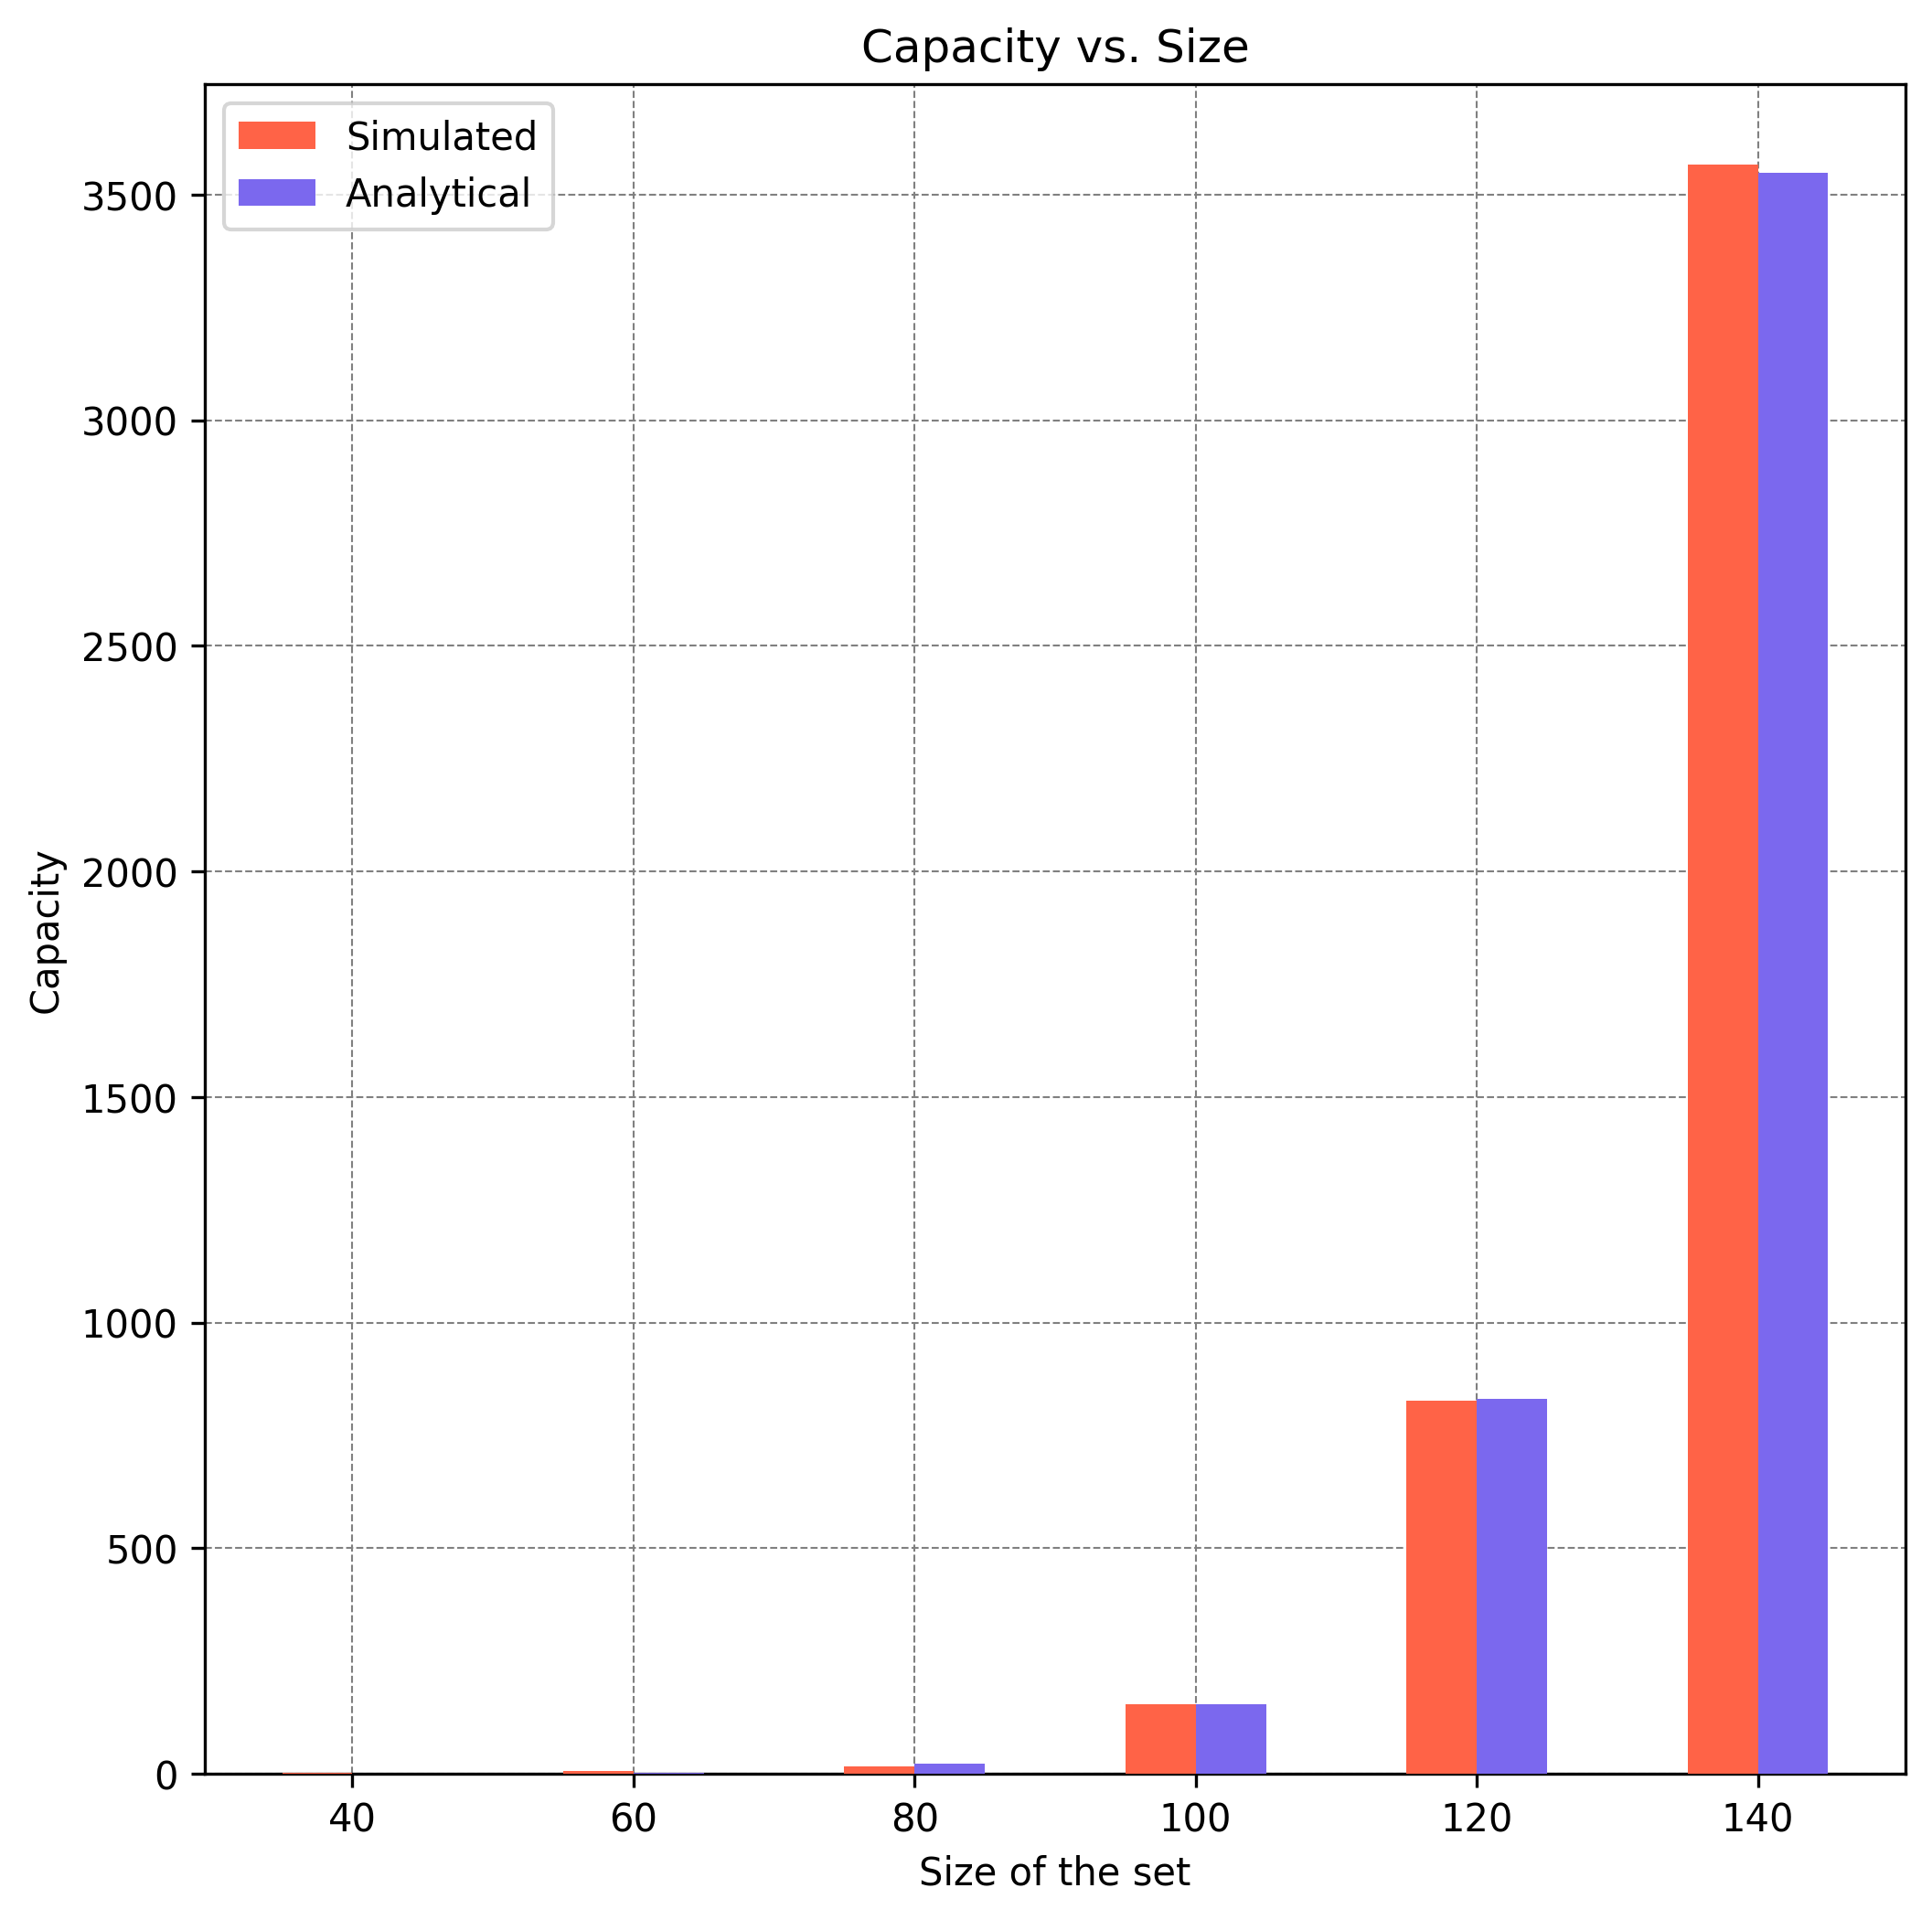
\includegraphics[scale=0.8]{figures/cap-vs-n.png}
    \caption[Capacity vs. Size of the set ($n$)]{Capacity vs. Size of the set ($n$). \textmd{How capacity is affected by increasing the size of the set ($n$). This figure compares the expression for fixed subset size against the simulation with fixed subset size.}}
    \label{figure:cap-vs-n}
    \end{figure}

We compare the average capacity of the simulation with the analytical result from Theorem \ref{thm:exact-r} as a function of the size of the set. We fix $r=20$, $k=2$, $T=0.1$. Figure \ref{figure:cap-vs-n} shows the results of this comparison. We see that the average simulated capacity is practically identical to the analytical capacity thoughout our input range.


    \begin{figure}%[h]
        \centering
        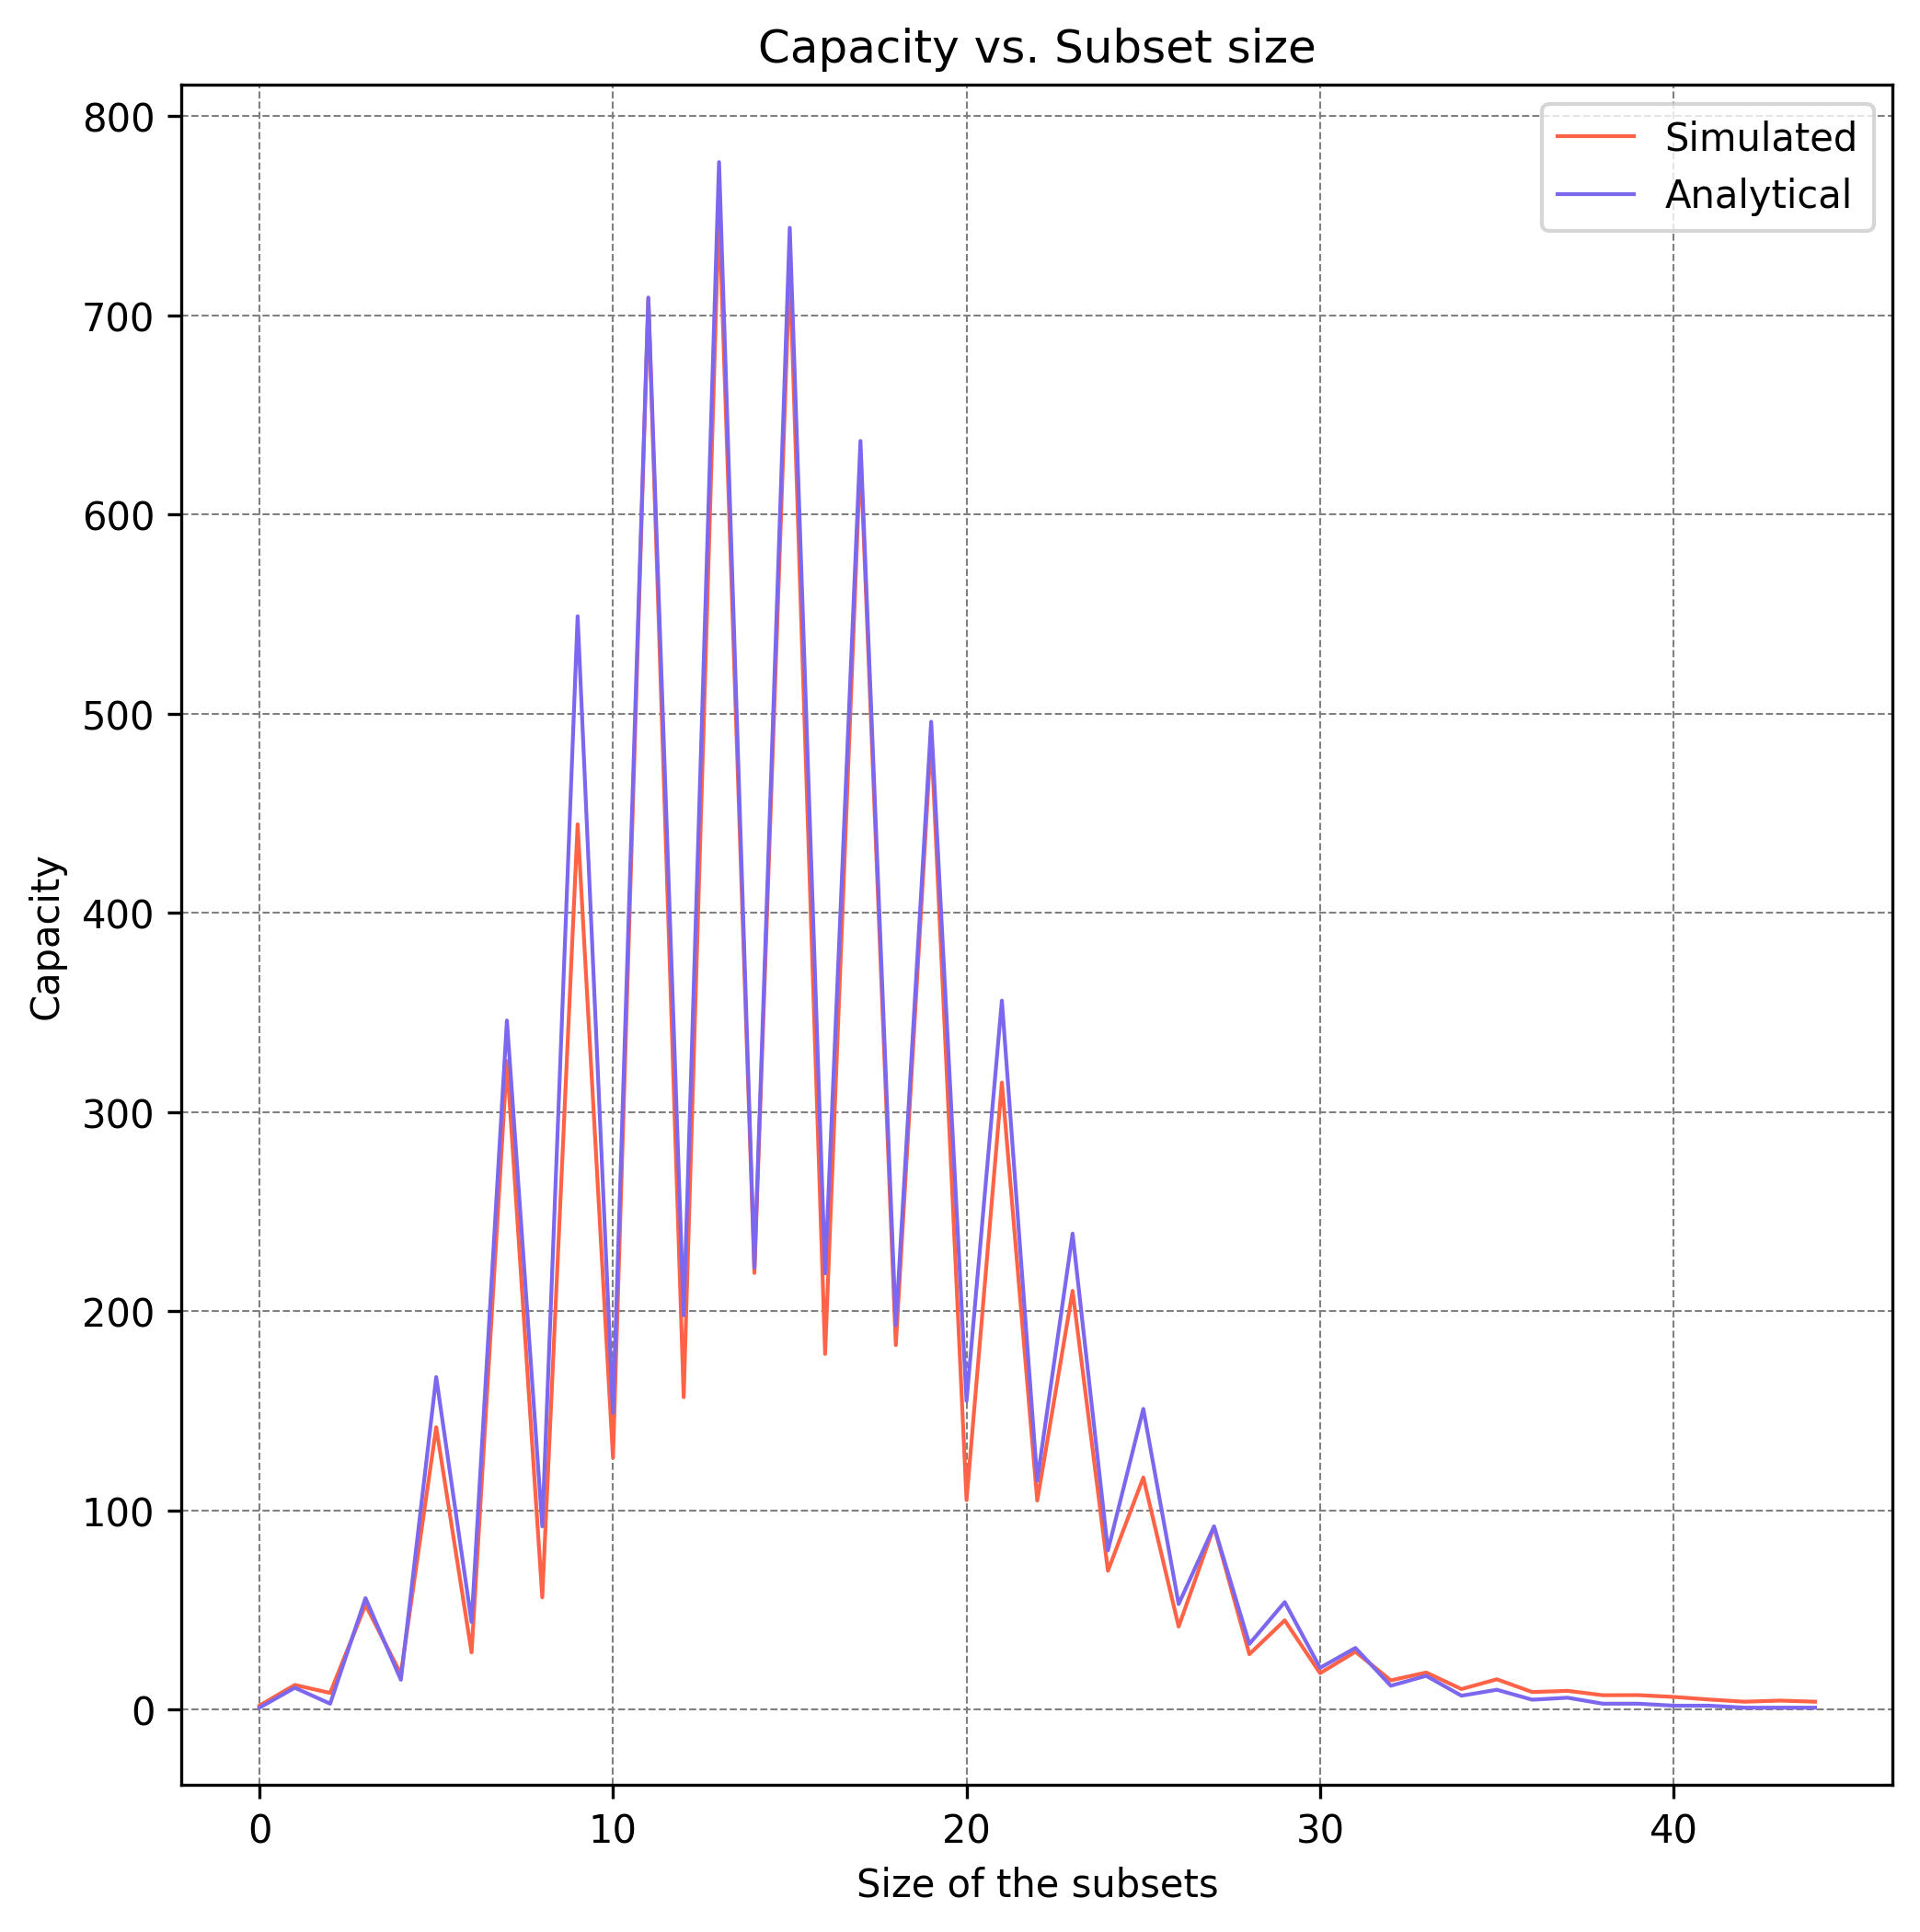
\includegraphics[scale=0.85]{figures/cap-vs-r.png}
        \caption[Capacity vs. Size of the subsets ($r$)]{Capacity vs. Size of the subsets ($r$). \textmd{How capacity is affected by increasing the size of the subsets ($r$). This figure compares the expression for fixed subset size against the simulation with fixed subset size.}}
        \label{figure:cap-vs-r}
        \end{figure}

    \begin{figure}%[h]
            \centering
            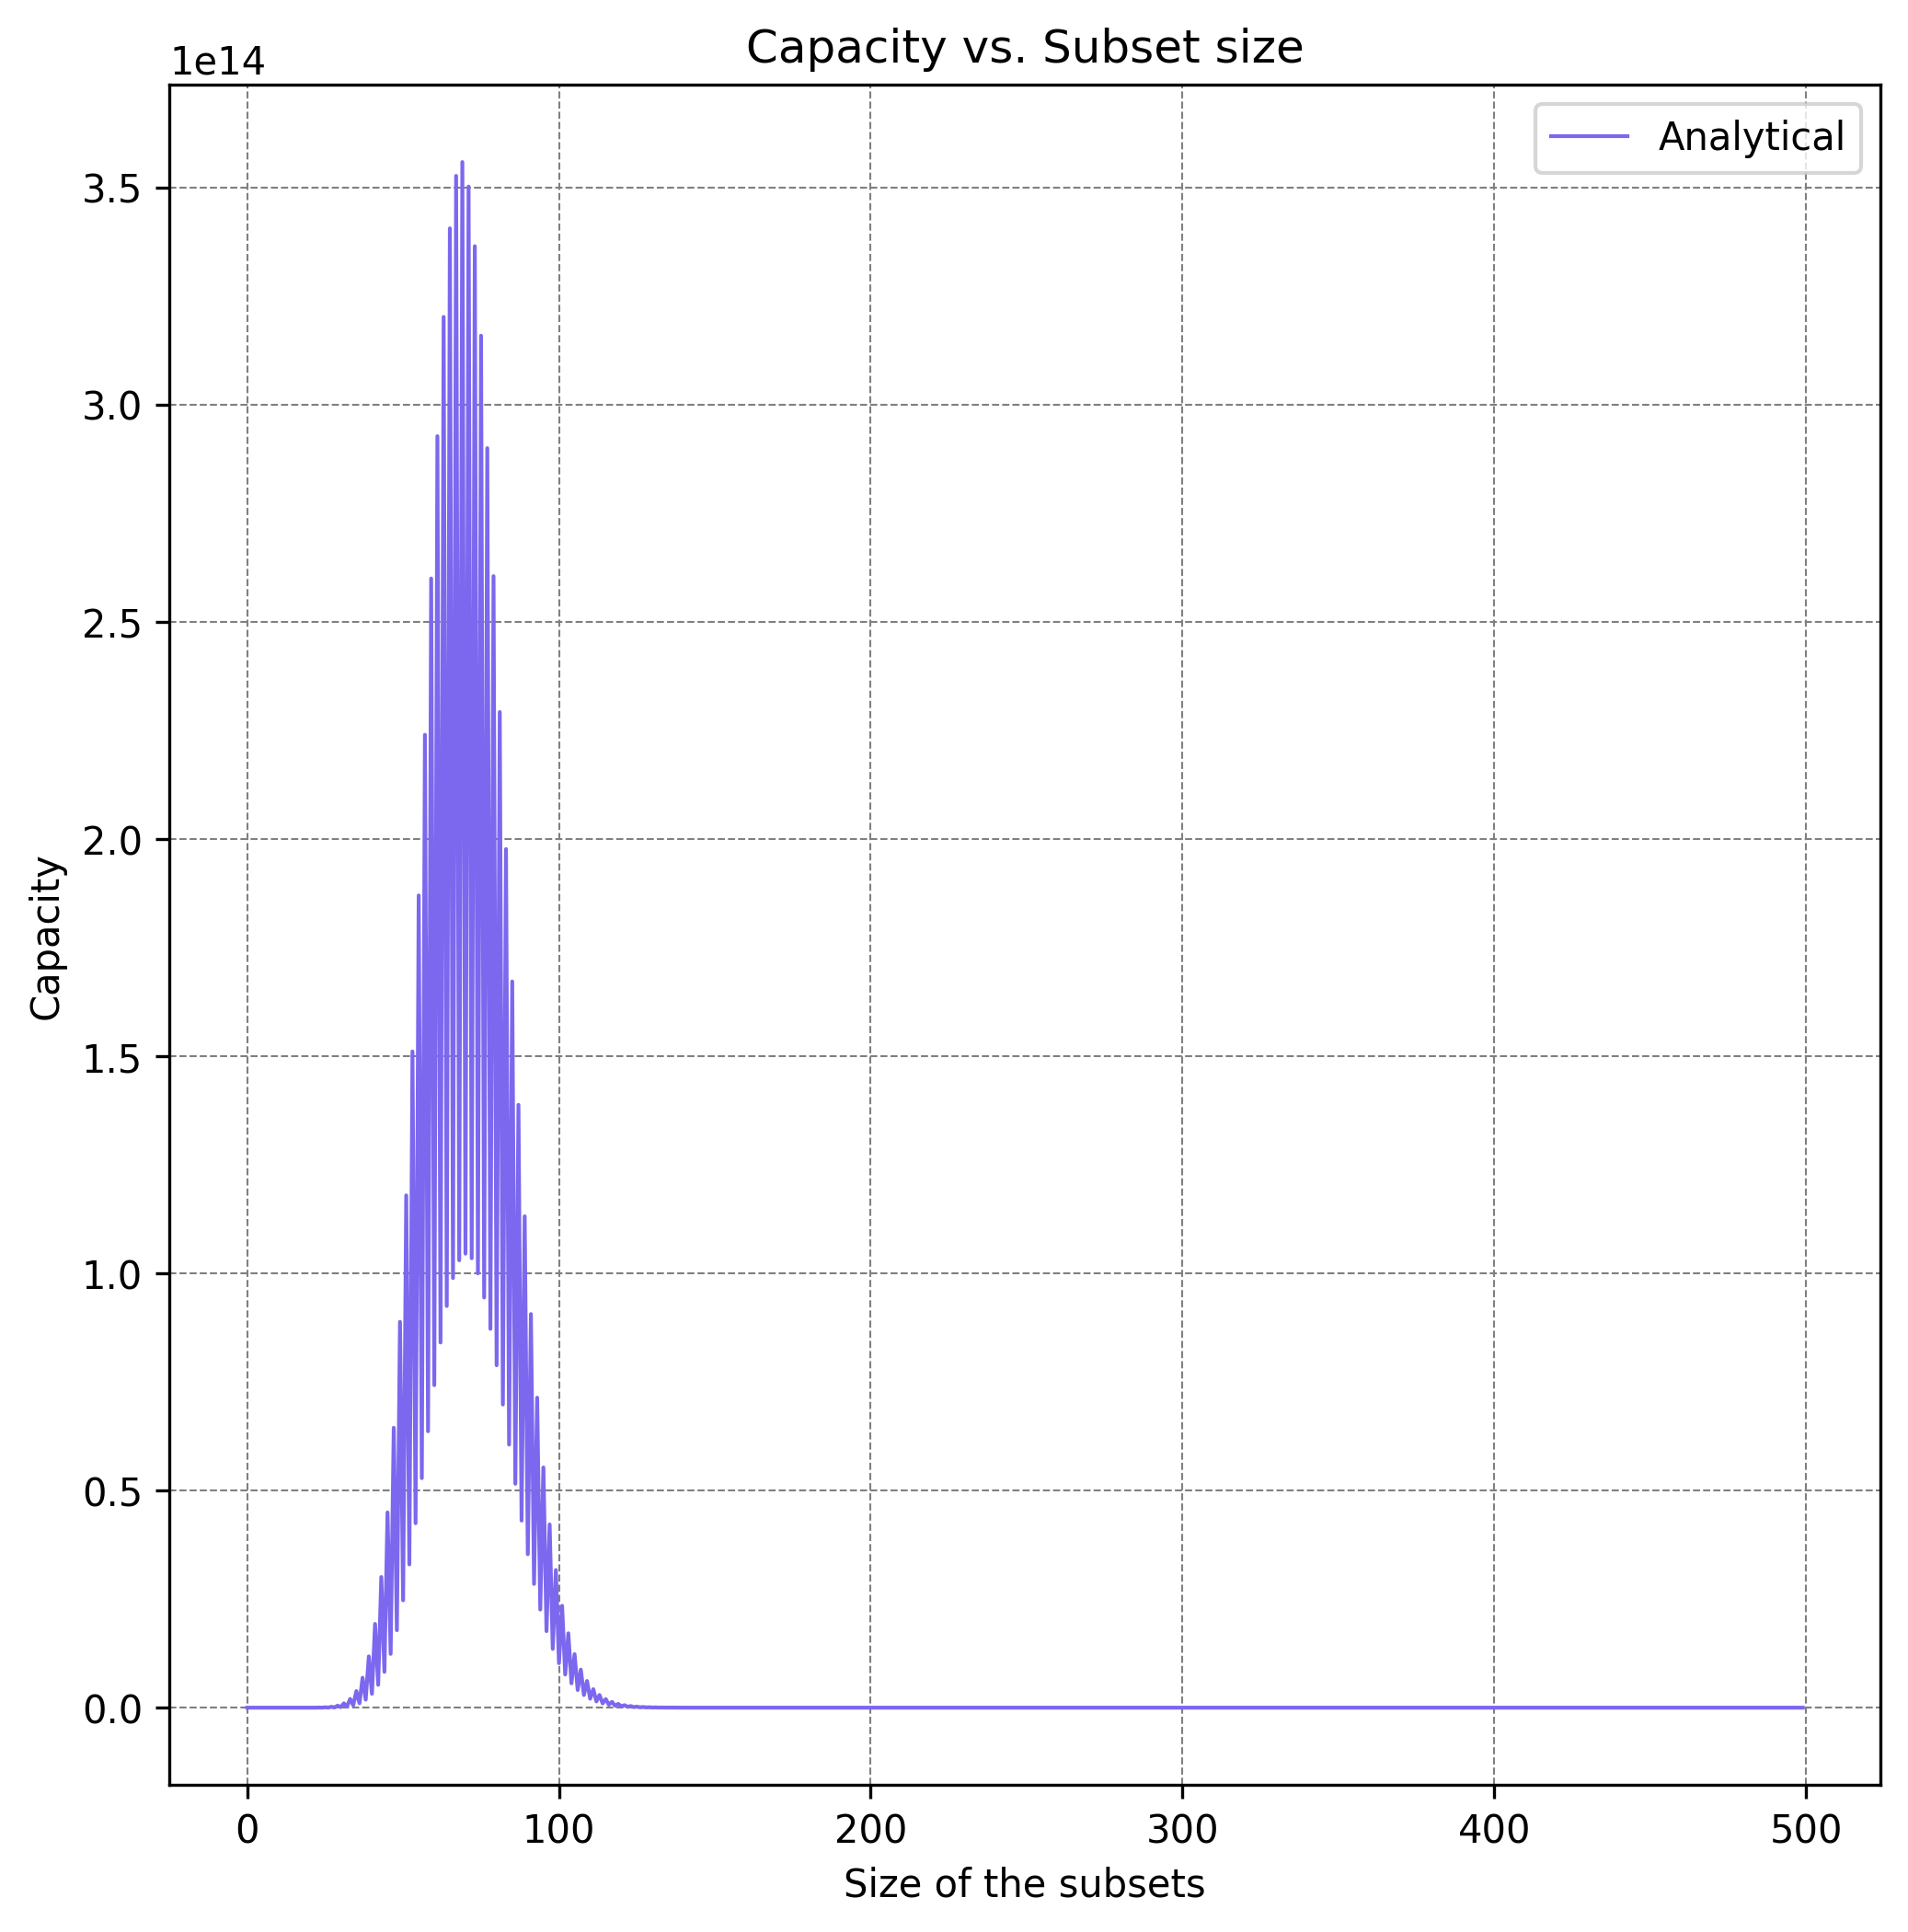
\includegraphics[scale=0.85]{figures/larger-n.png}
            \caption[Capacity vs. Size of the subsets ($r$) for $n = 500$]{Capacity vs. Size of the subsets ($r$) for $n = 500$. \textmd{How capacity is affected by increasing the size of the subsets ($r$) when $n = 500$.}}
            \label{figure:larger-n}
            \end{figure}

Then we the compare the average capacity of the simulation with the analytical result from Theorem \ref{thm:exact-r} as a function of the size of the subsets $r$. We fix $n=100$, $k=2$, $T=0.1$. Figure \ref{figure:cap-vs-r} shows the results of this comparison. We see that the average simulated capacity is very close to the analytical capacity thoughout our input range and follows the general trend, even following the sharp decreases while going from odd numbers to even numbers. This is because the sets need intersections of size atleast $\lceil r/2 \rceil$ to interfere and as the size of the subset goes from an odd number to the next even number, this value remains the same while the size of the subsets increase leading to a higher probability of interference and lower capacity. One can also think of it as more terms being included in the sum in Lemma \ref{lemma:k-int-prob}. We believe these peaks will reduce in intensity relative to the scale of the y axis as $n \to \infty$. Figure \ref{figure:larger-n} shows the values of analytical capacity with same configuration as above but with n set to 500. We can already see that the graph has become a lot smoother. Unfortunately, it is impossible for us to simulate models of this size or bigger due to memory constraints. 

\subsection{Bounded subset size}
Now we simulate the case where the subset sizes are not fixed but rather bounded above and below. 

\begin{figure}%[h]
    \centering
    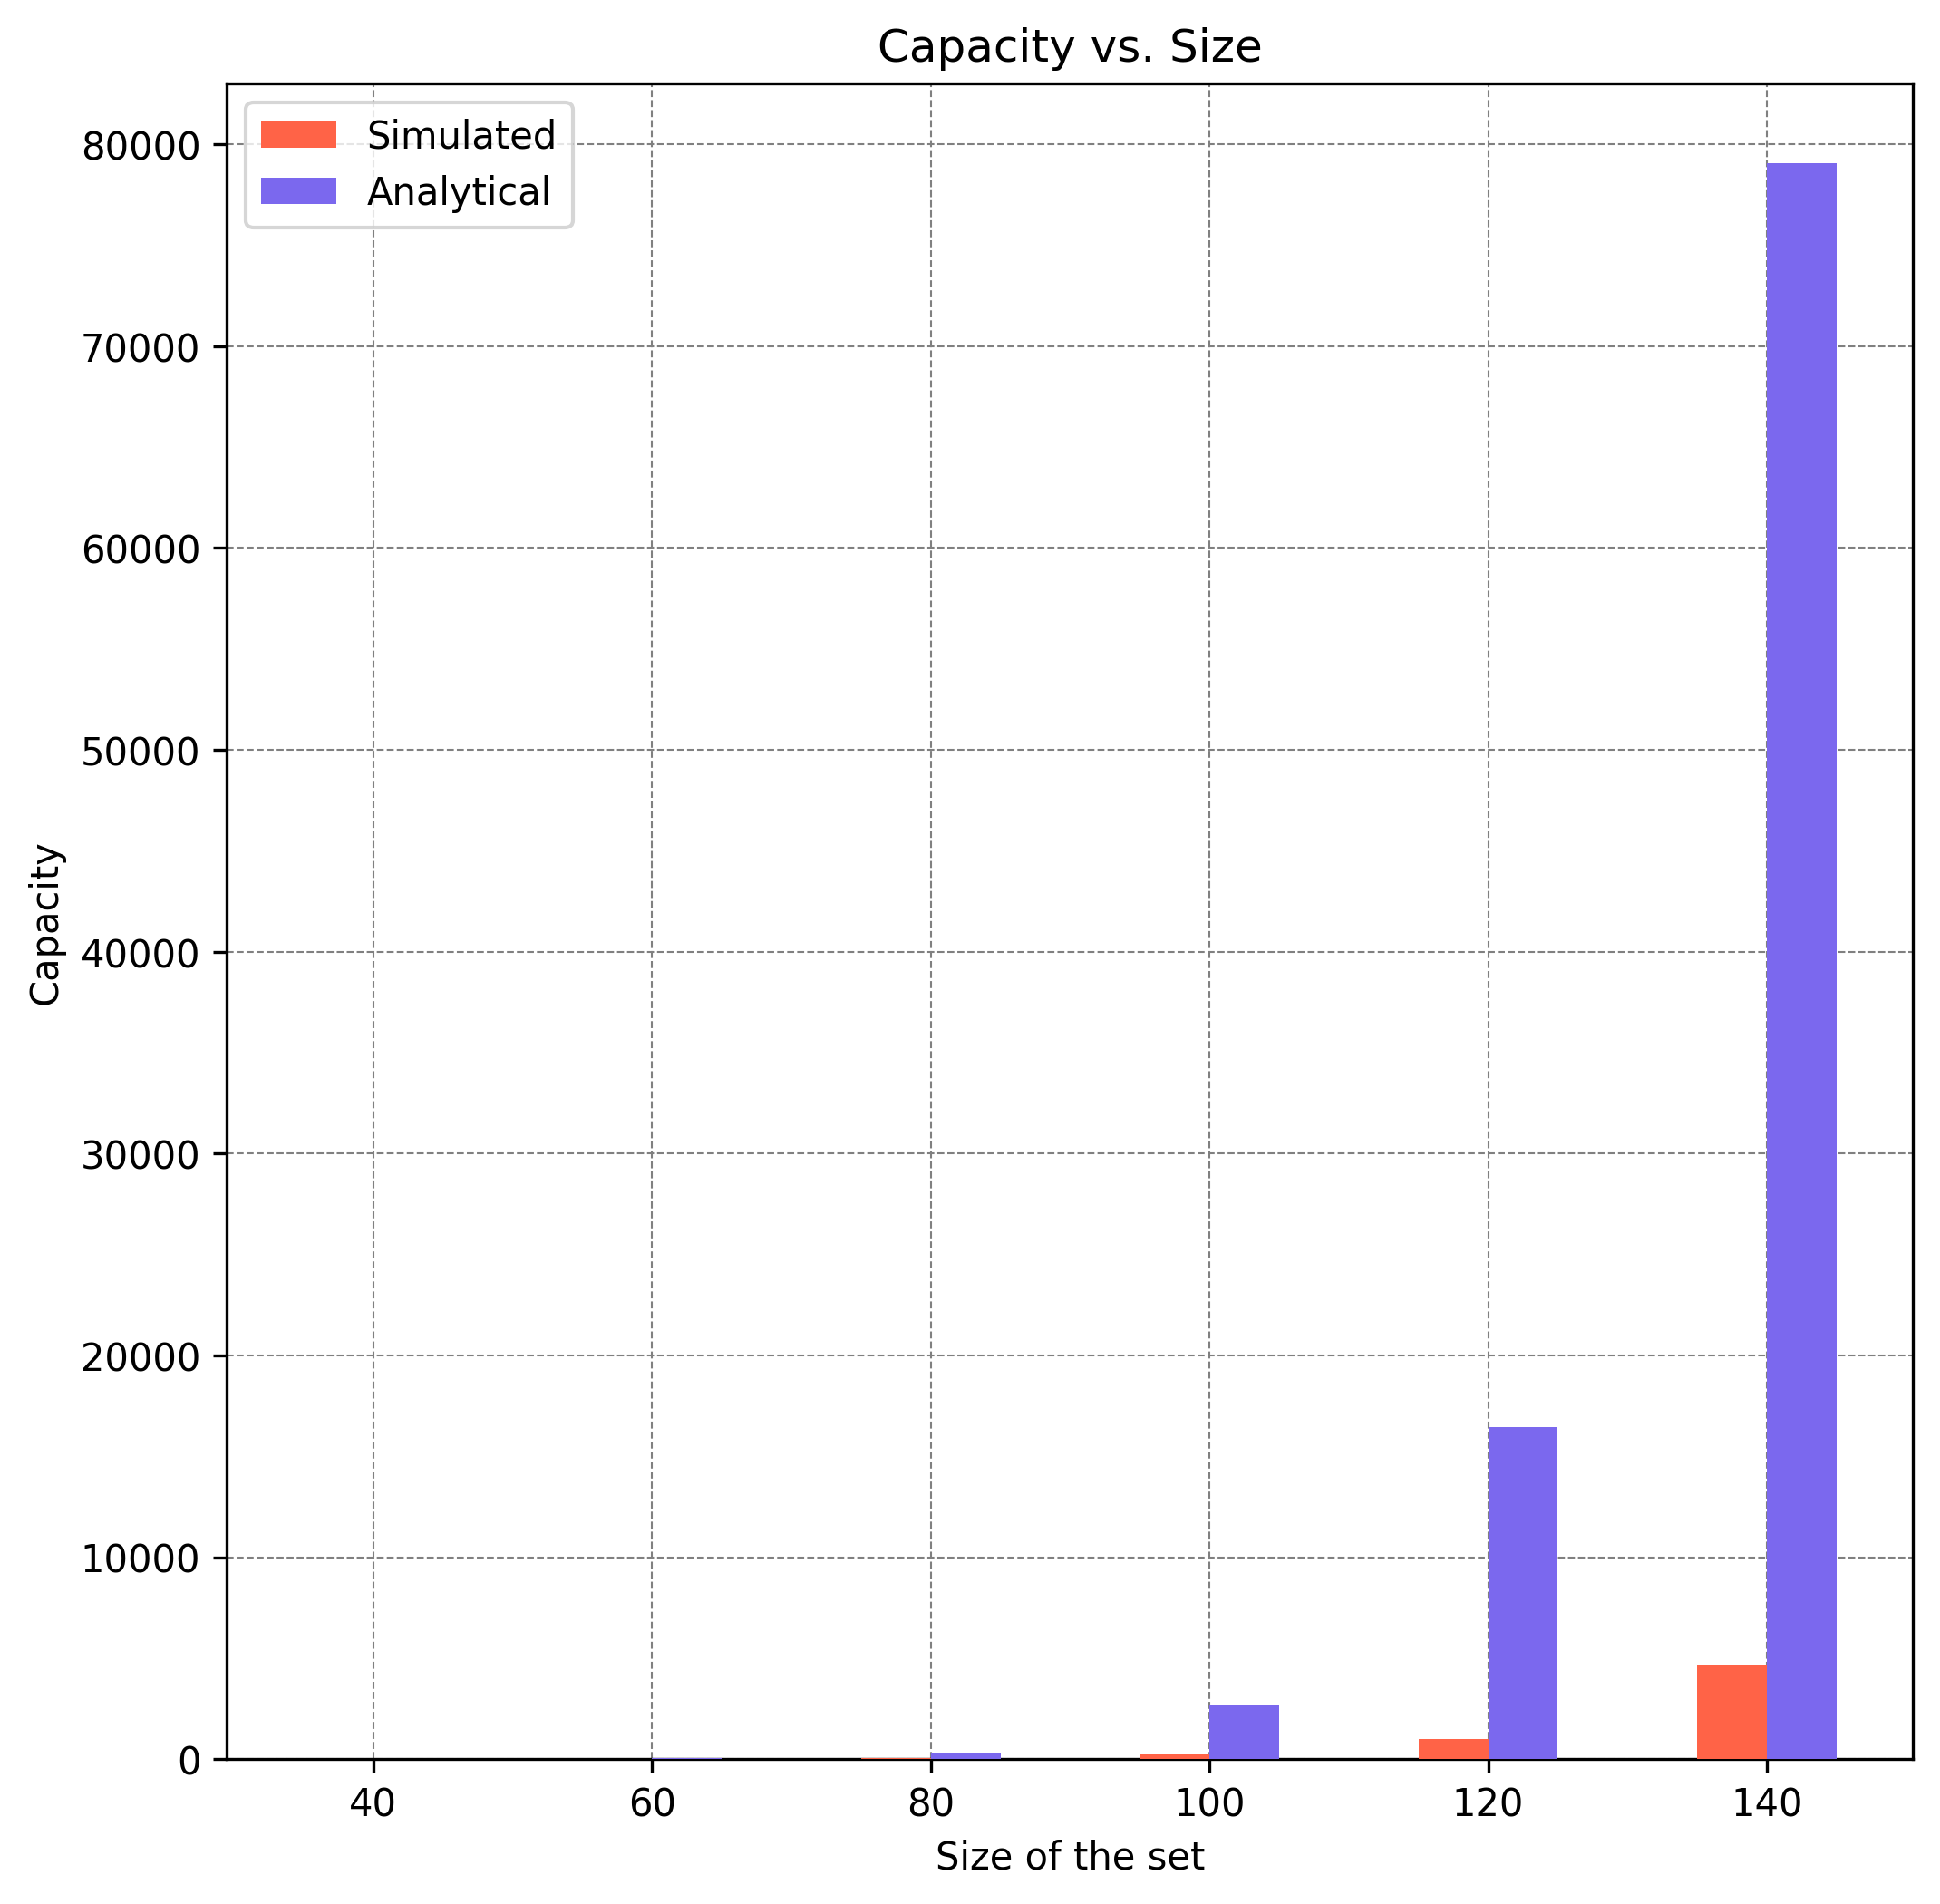
\includegraphics[scale=0.82]{figures/cap-vs-n-bounded.png}
    \caption[Capacity vs. Size of the set ($n$) when $r \sim \mathcal{N}(r,1)$]{Capacity vs. Size of the set ($n$) when $r \sim \mathcal{N}(r,1)$. \textmd{How capacity is affected by increasing the size of the subsets ($r$) when $r$ is drawn from a normal distribution with mean $r$ and standard deviation $1$. This figure compares the expression for bounded subset size against the simulation that draws memories from a distribution.}}
    \label{figure:cap-vs-n-bounded}
    \end{figure}

\begin{figure}%[h]
    \centering
    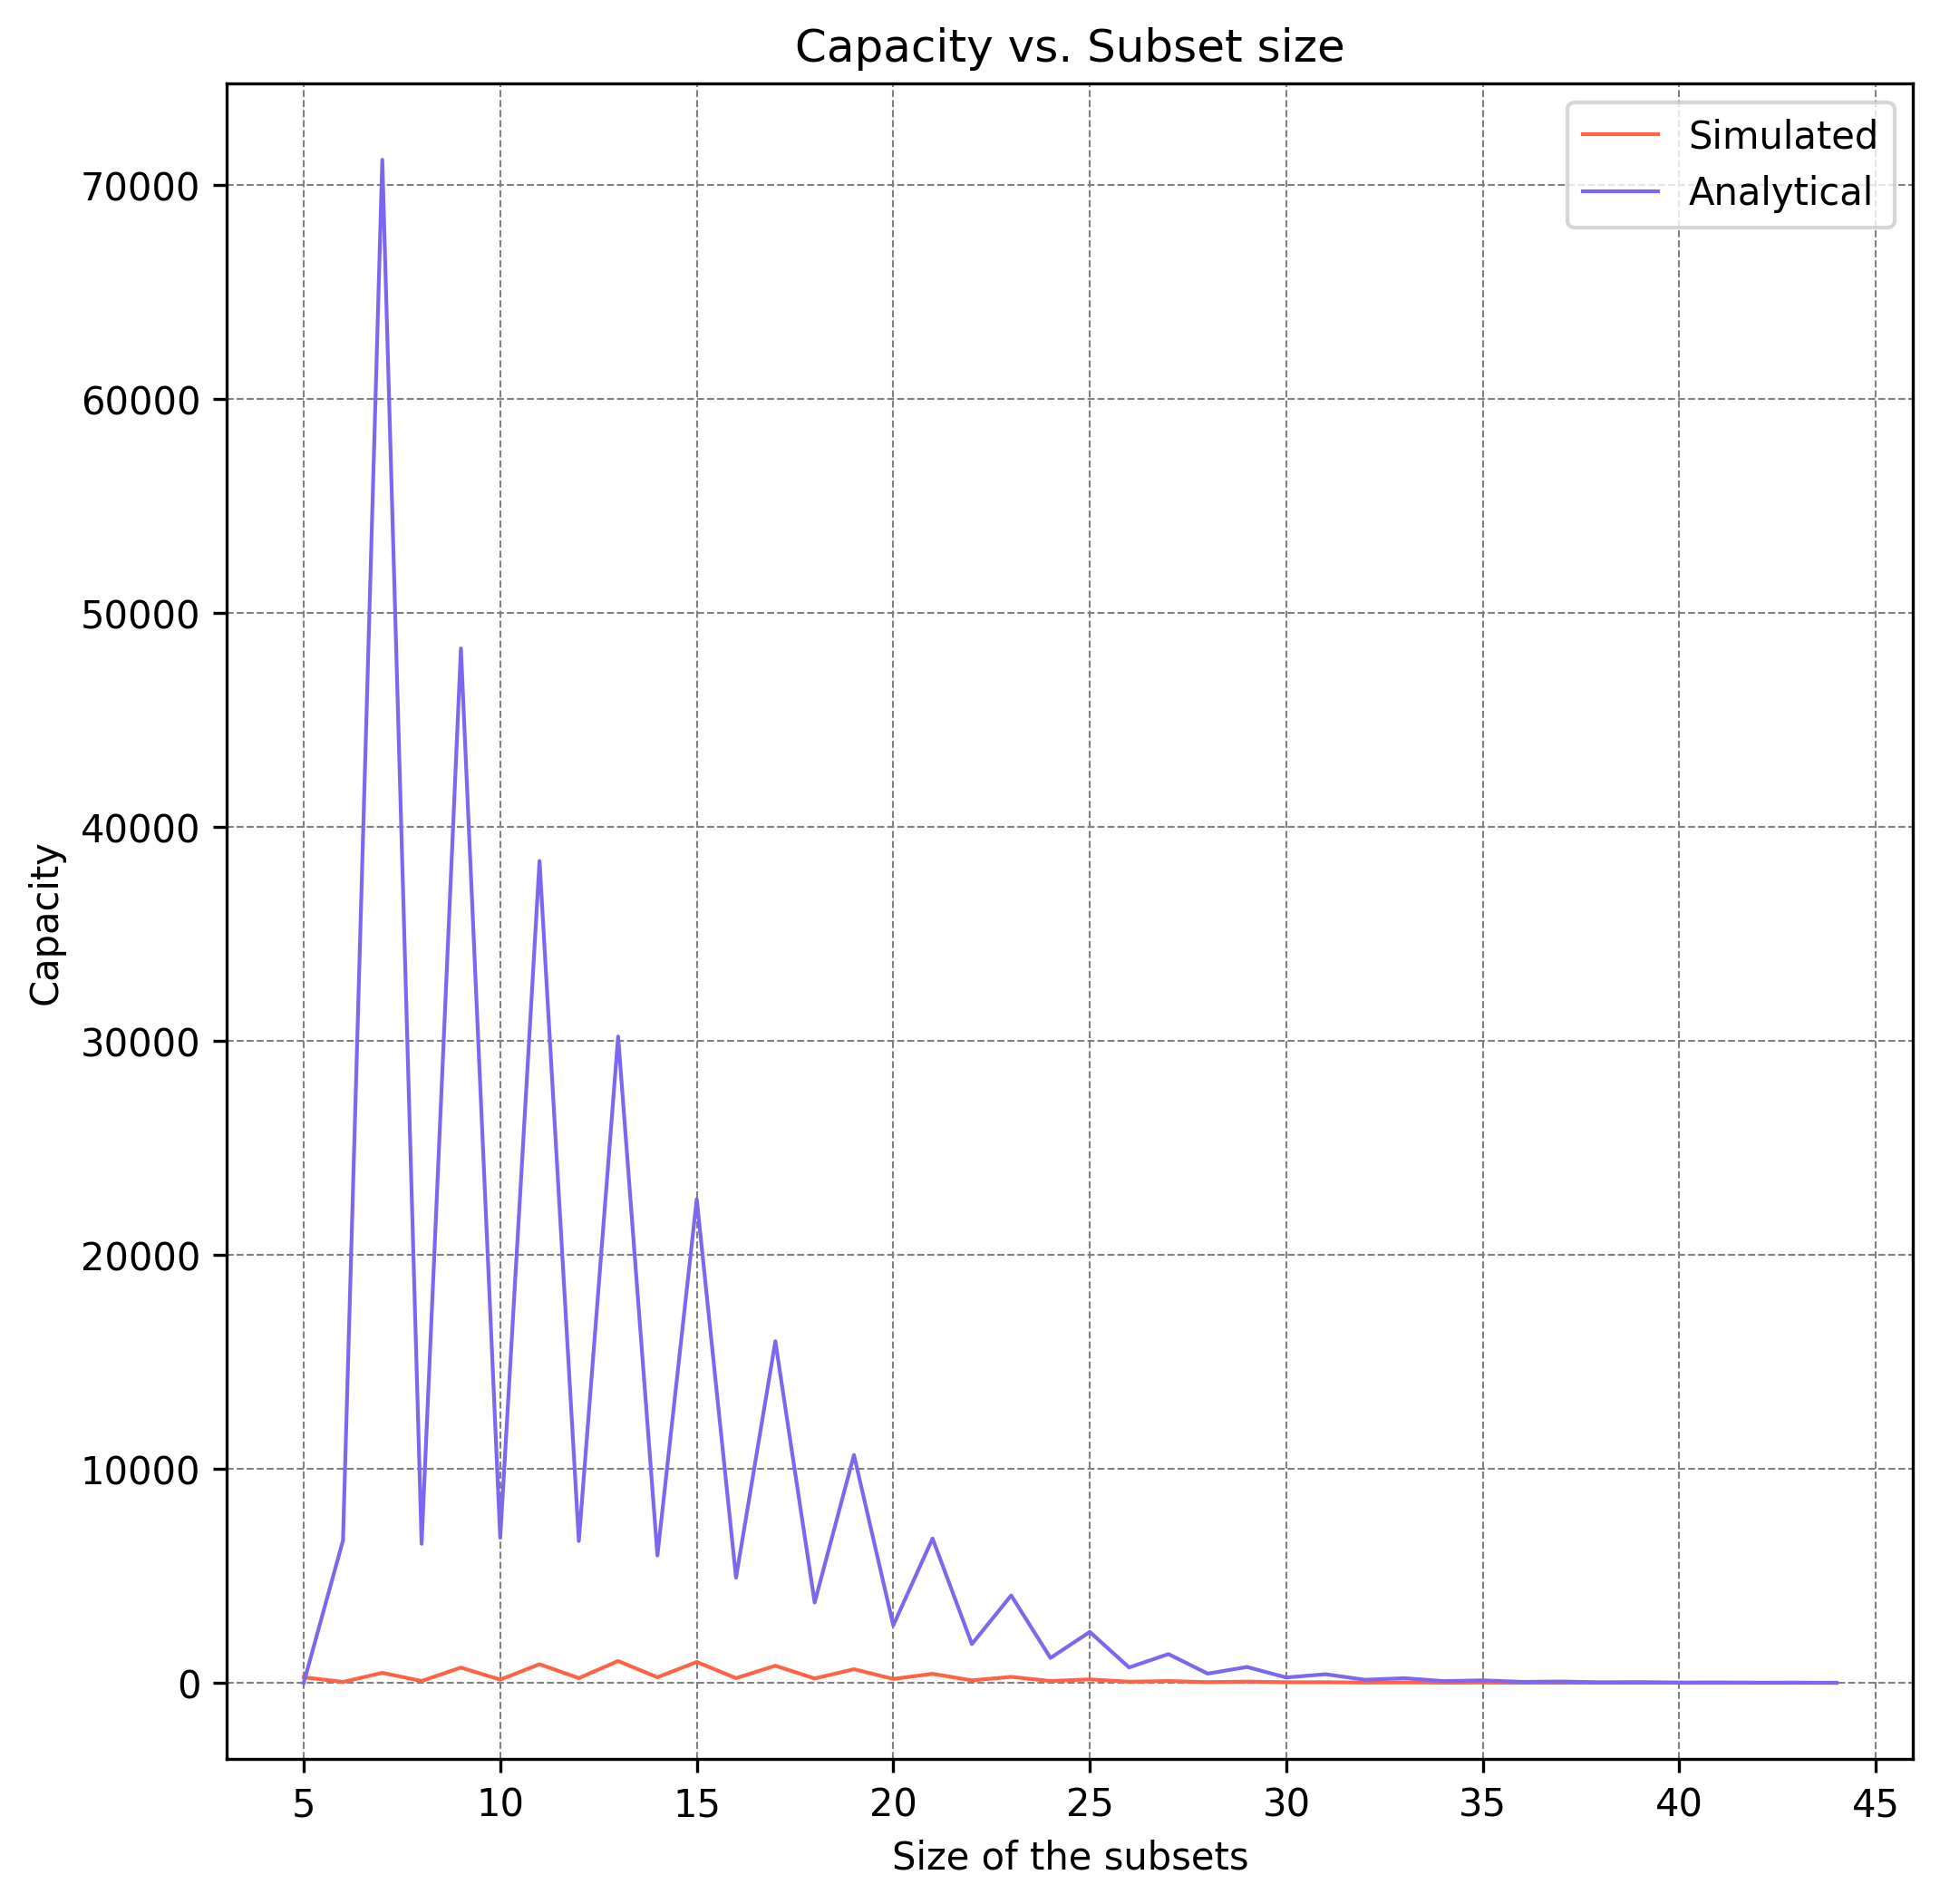
\includegraphics[scale=0.83]{figures/cap-vs-r-bounded.png}
    \caption[Capacity vs. Size of the subsets ($r$) when $r \sim \mathcal{N}(r,1)$]{Capacity vs. Size of the subsets ($r$) when $r \sim \mathcal{N}(r,1)$. \textmd{How capacity is affected by increasing the size of the subsets ($r$) when $r$ is drawn from a normal distribution with mean $r$ and standard deviation $1$. This figure compares the expression for bounded subset size against the simulation that draws memories from a distribution.}}
    \label{figure:cap-vs-r-bounded}
    \end{figure}

    \begin{figure}%[h]
        \centering
        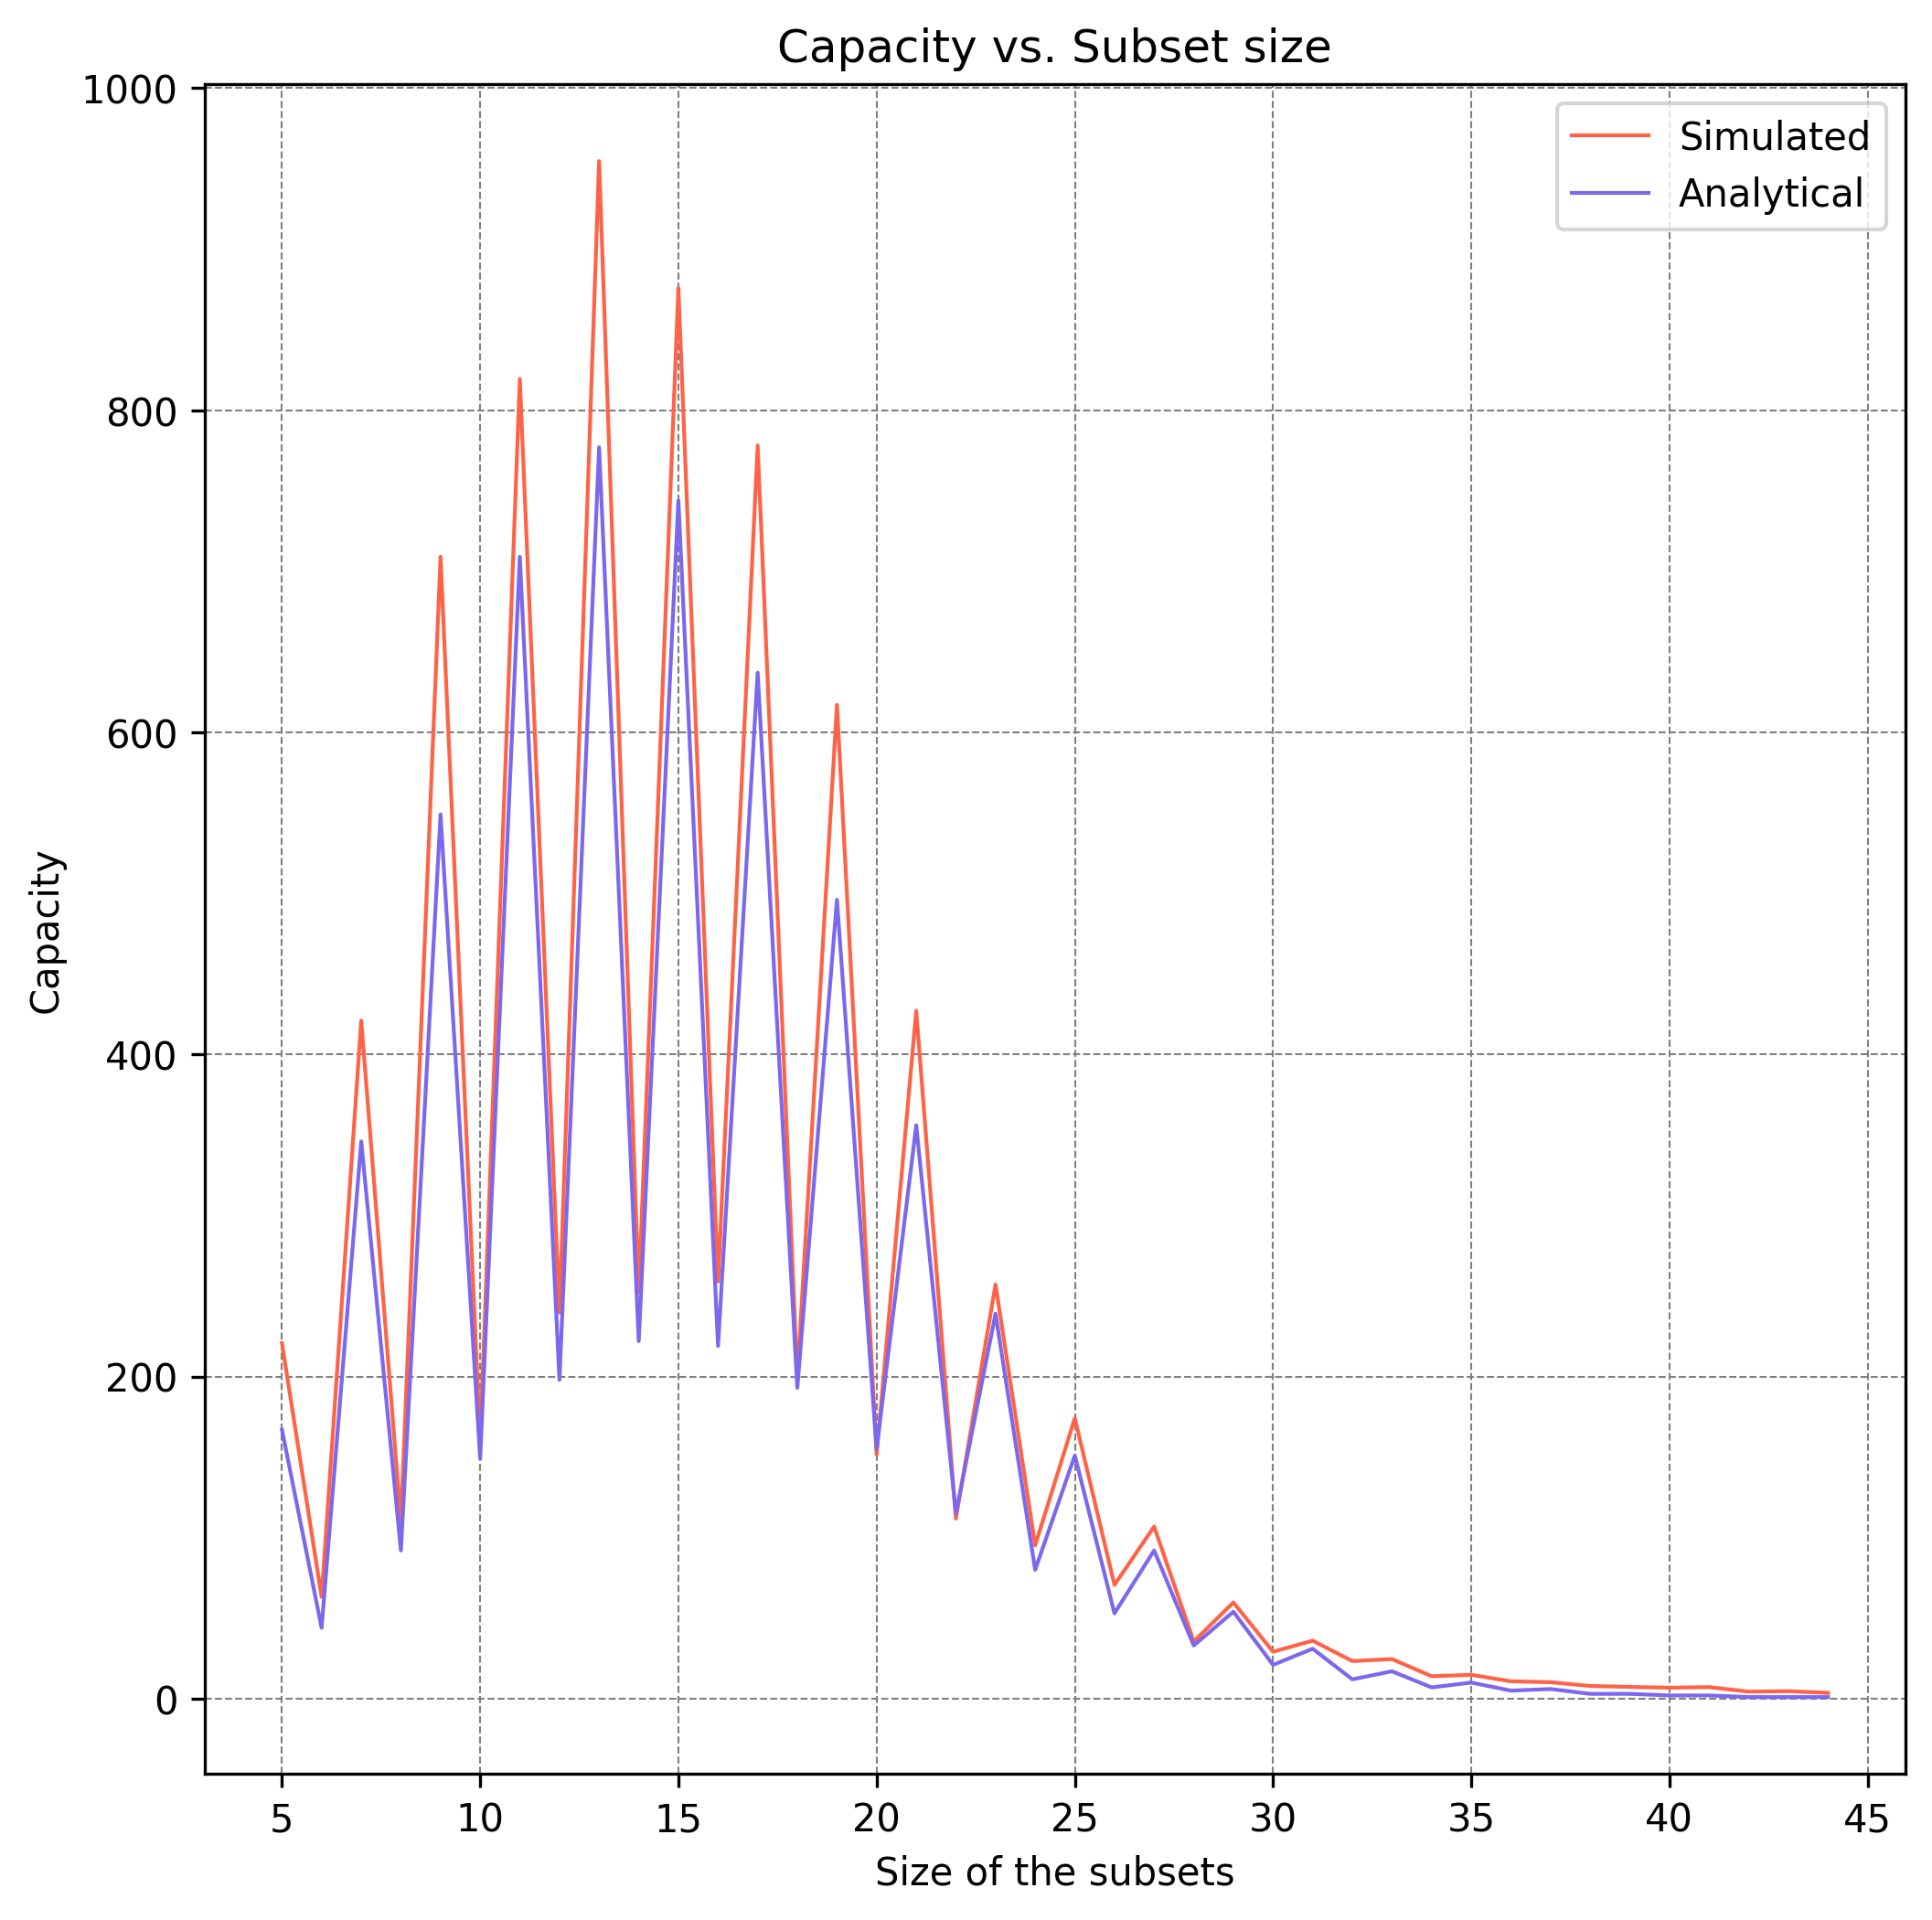
\includegraphics[scale=0.83]{figures/cap-vs-r-bounded-exact-1.png}
        \caption[Capacity vs. Size of the subsets ($r$) when $r \sim \mathcal{N}(r,1)$ comparing exact formula vs simulation]{Capacity vs. Size of the subsets ($r$) when $r \sim \mathcal{N}(r,1)$ comparing exact formula vs simulation. \textmd{How capacity is affected by increasing the size of the subsets ($r$) comparing the results of \ref{equ:cap-exact-r} with the simulation where $r$ is drawn from a normal distribution with mean $r$ and standard deviation $1$. This figure compares the expression for fixed subset size against the simulation that draws memories from a distribution.}}
        \label{figure:cap-vs-r-bounded-exact-1}
        \end{figure}

        \begin{figure}%[h]
            \centering
            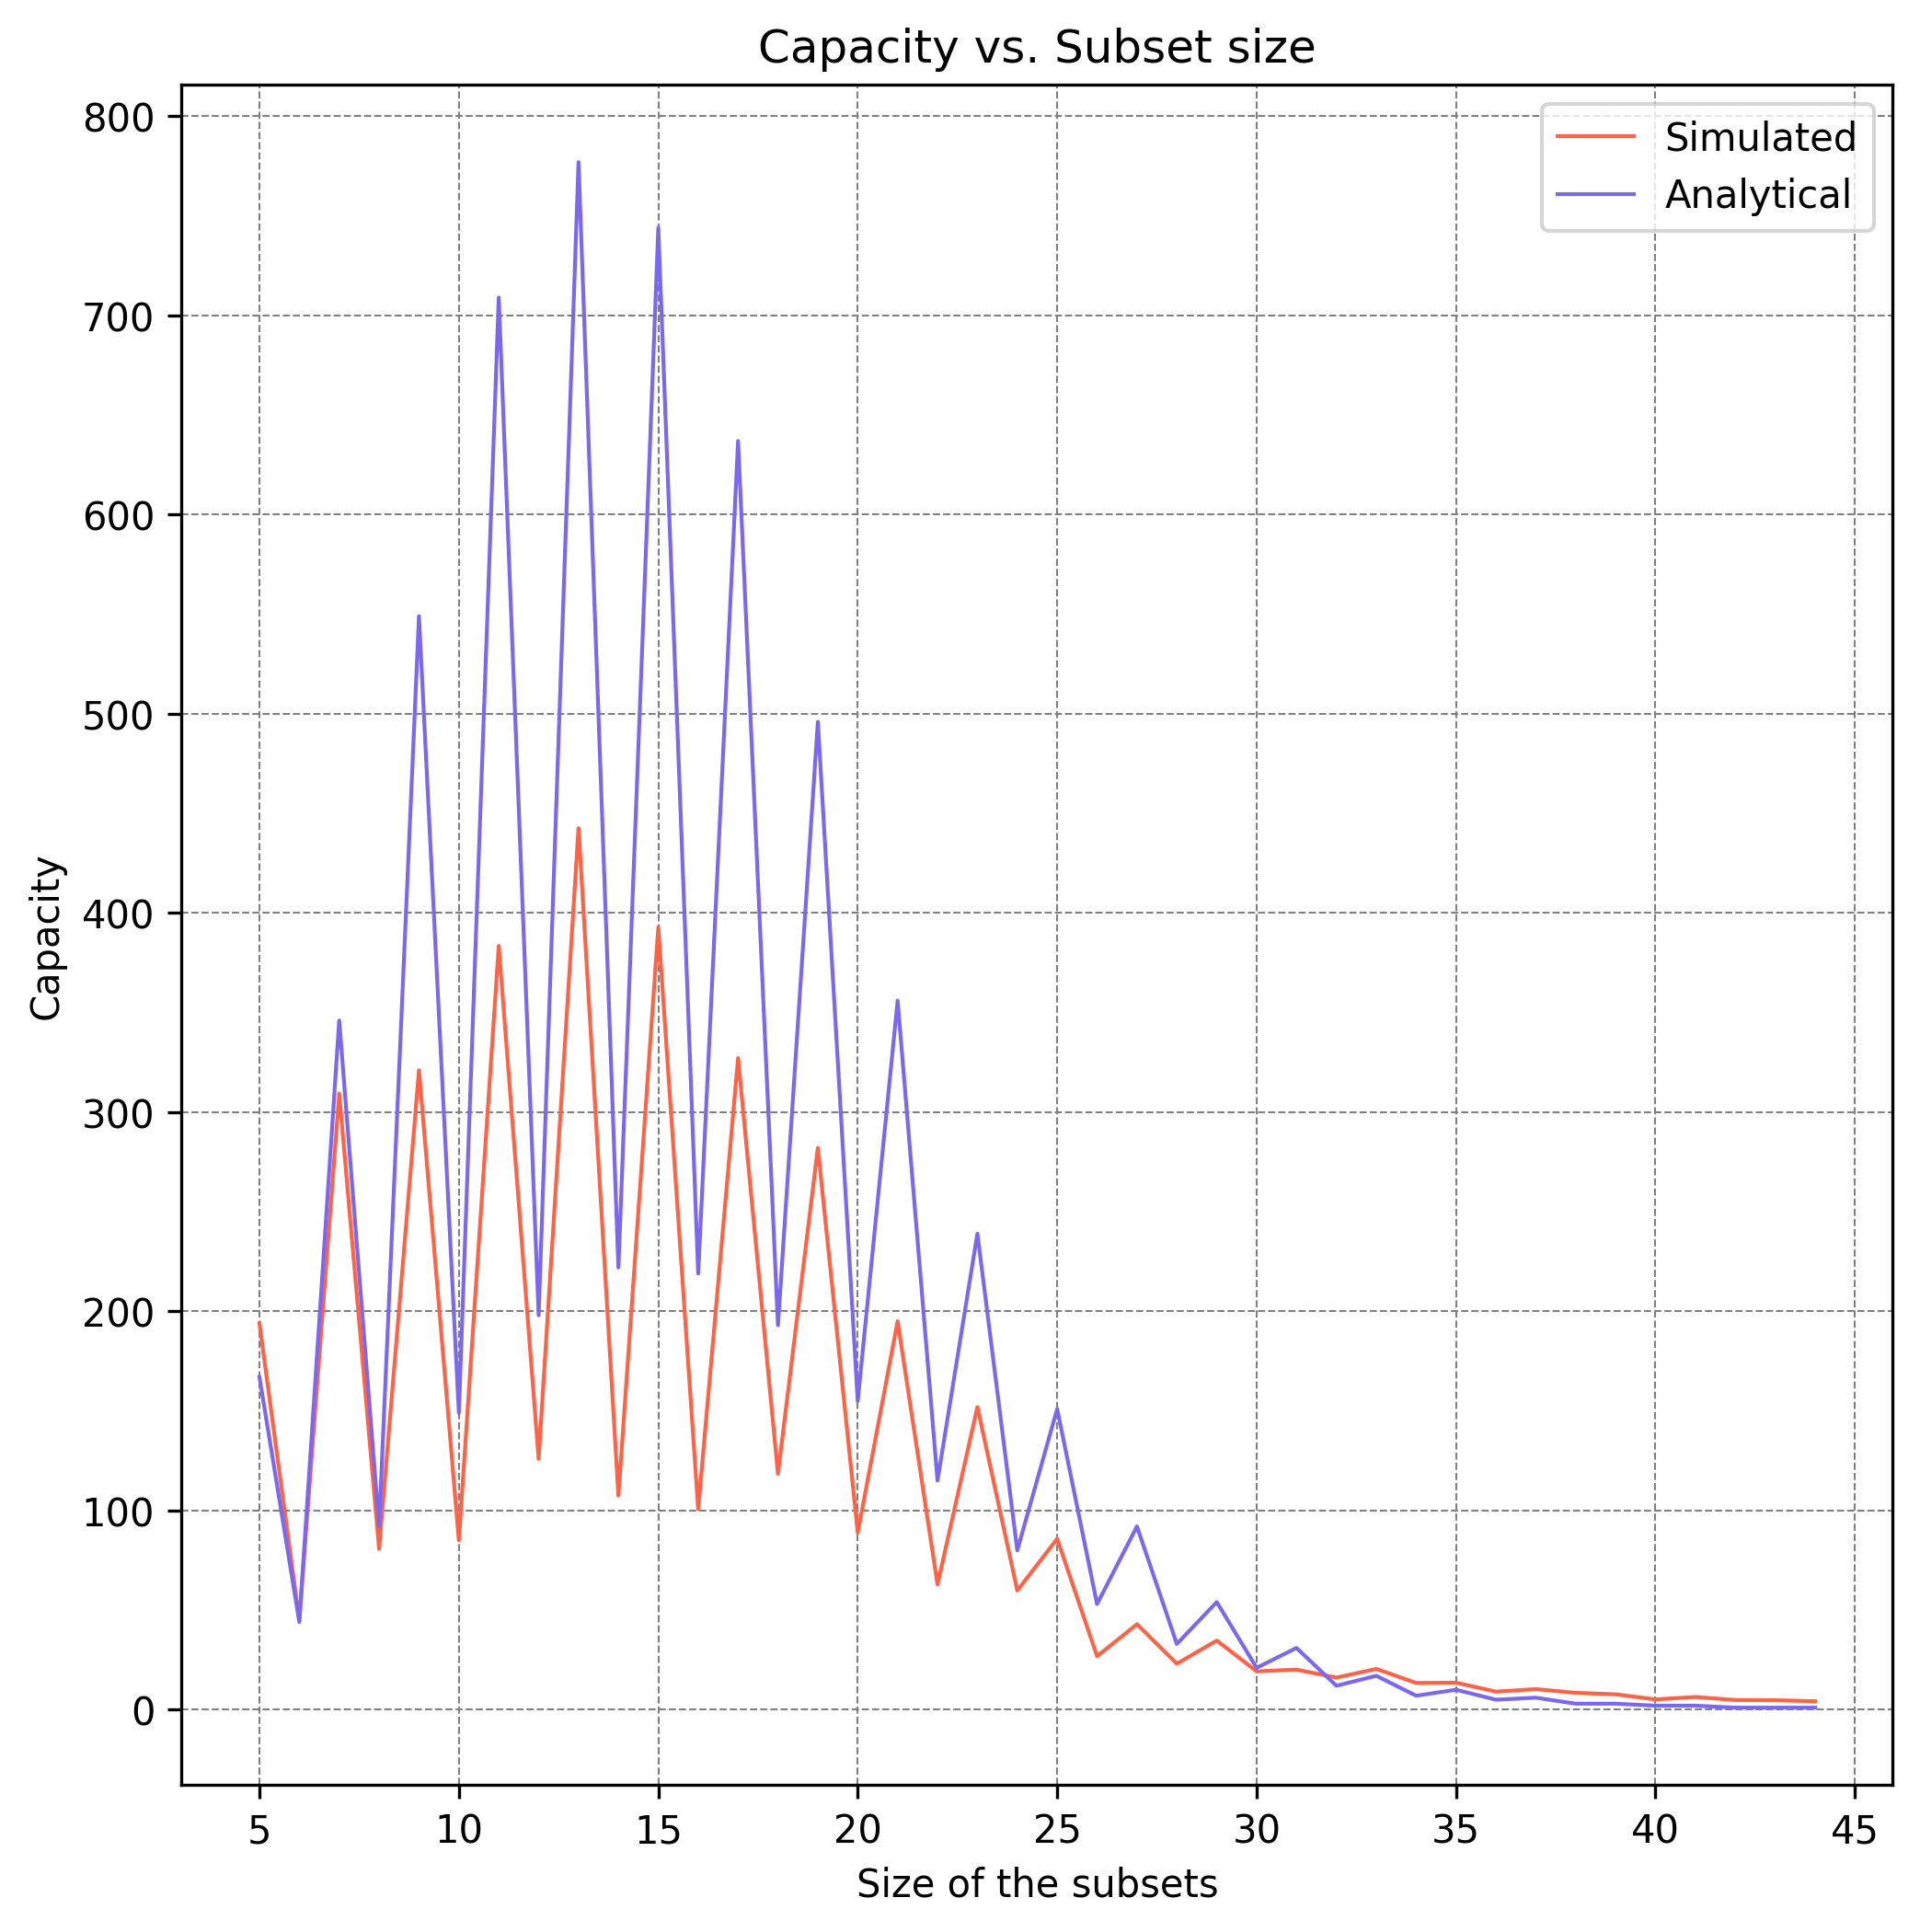
\includegraphics[scale=0.83]{figures/cap-vs-r-bounded-exact-2.png}
            \caption[Capacity vs. Size of the subsets ($r$) when $r \sim \mathcal{N}(r,2)$]{Capacity vs. Size of the subsets ($r$) when $r \sim \mathcal{N}(r,2)$. \textmd{How capacity is affected by increasing the size of the subsets ($r$) comparing the results of \ref{equ:cap-exact-r} with the simulation where $r$ is drawn from a normal distribution with mean $r$ and standard deviation $2$. This figure compares the expression for fixed subset size against the simulation that draws memories from a distribution.}}
            \label{figure:cap-vs-r-bounded-exact-2}
            \end{figure}

Like in the fixed case, we compare the simulated and analytical capacities against the size of the set and against the size of the subsets. For the comarison against size of the set, we set $r = 20$ and for the comparison against size of the subsets, we set $n = 100$. For both cases we fix $k=2, T=0.1$ and draw the $r$ values randomly from $\mathcal{N}(r,1)$ followed by conversion to integer. Based on the Empirical Law, we except $95\%$ of the values to lie within two standard deviations of $r$, so we choose $\delta = 2$. Figures \ref{figure:cap-vs-n-bounded} and \ref{figure:cap-vs-r-bounded} show the results of these experiments. We see that even thought the analytical bound from equation \ref{equ:cap-bound-expected} bounds the simulated capacity, the bound is very loose and does cannot be used as an approximation. We believe this is because of how the binomial coefficient varies with respect to its second parameter and that $\delta$ here, even though only $2$ is quite big with respect to $r$, and is reducing the second argument significantly in the term $n - r - \delta \choose r - \delta - y$. We believe that a larger $n$ and $r$ will make this bound tighter and applications like the Neuroidal model indeed use values of $n$ and $r$ that are orders of magnitudes larger. However, it is not feasible for us to simulate at such scale. We also compared the analytical results from equation \ref{equ:cap-exact-r} and it was still a good approximation for the simulation with randomly drawn r's. Figures \ref{figure:cap-vs-r-bounded-exact-1} and \ref{figure:cap-vs-r-bounded-exact-2} show the results of these simulations. As expected the simulated capacity is a lot closer to the analytical capacity when the standard deviation is low. 

\section{Discussion}

We believe our theoretical framework for interference and capacity calculations can be extended to analyze and understand the behavior of graph-based models with more complex memory creation algorithms. The primary distinction between our simple model and more complicated models like the Neuroidal model and Assembly Caculus is with regards to the memory creation algorithm. We implicitly assume a random memory creation algorithm in lemma \ref{lemma:k-int-prob} while the Neuroidal model uses the JOIN operation and the Assembly Calculus uses the Project and Merge operations for memory creation \cite{papadimitriou2020brain, valiant2005memorization}. Since no other part of our theory makes any assumption about the process of memory formation, we believe that adjusting the calculation of expected interference between two memories in lemma \ref{lemma:k-int-prob} to incorporate the nuances of other memory creation algorithms and using it appropriately in Theorem \ref{thm:exact-r} or \ref{thm:bounded-r} will give us an accurate representation of capacity in those models.

We maintain the generality of our interference calculation while allowing for variations in memory creation algorithms. Specifically, we can refine the lemma to account for the JOIN, Project and Merge operations, ensuring that our interference metric aligns with the unique characteristics of each model. This adaptability enables the application of our interference and capacity framework to a broader class of graph-based models in computational neuroscience.

The flexibility of our theoretical approach allows researchers to tailor interference calculations based on the specifics of memory creation algorithms in diverse neural network models. As a result, our capacity analysis can provide valuable insights into the limitations and efficiency of these models, enhancing our understanding of their memory storage capabilities.

\subsection{Capacity and JOIN}

In this section, we briefly discuss some insights we gained from our analysis of the JOIN operation with regards to capacity. 

The JOIN algorithm is unique in the sense that it must follow a set of 6 basic constraints which ensure that the newly formed memories are roughly the same size as the memories that were JOINed and therefore the size of the memories ($r$) remains more or less fixed for a given graph size ($n$), expected degree ($d$) and edge weight $(w)$. Note that edge degree and synaptic weight were not a factor in our theory as edges do not matter when memories are randomly inserted. However, we believe that an updated JOIN-compliant formula expected interference between two memories will involve these paramters. 

First, we compare our results from equation \ref{equ:cap-bound-expected} with results from our simulation of the Neuroidal Model. Valiant calculated the memory sizes for various parameter combinations, however the minimum graph size he considered was 100,000. Our simulation of the Neuroidal model cannot be scaled up that far so we use $n = 500, d = 128, w = 16$. We used patterns found in his results to estimate that $r = 40$ would be the appropriate value for this configuration. We start with 100 randomly generated memories which have negligible interference between them, essentially agreeing with our results from Theorem \ref{thm:bounded-r}. We observed that newly formed memories had sizes around $40$, validating that we are compliant with Valiant's definition of JOIN. Finally, we set the interference threshold $T = 0.1$ and interference parameter $k = 2$ as that is the only value of $k$ supported by the Neuroidal model. 

Our equation produces a capacity of 3203070686178 while the Neuroidal model simulation only reaches around 250 memories over 20 runs before stopping due to excess interference. Therefore our equation in its current form cannot serve as a good approximation for the Neuroidal model's capacity however it is effectively a very loose upper bound on most models like these as the memory formation is not capacity optimized which we think makes sense biologically. We believe random memory generation is quite good for capacity and memory formation algorithms that are even further optimized for capacity will be even more biologically implausible. As described in section 5.2.3, the theory will need to be updated to account for JOIN's behavior. 

Finally, we made some attempts to gain some initial understanding of why memories formed by JOIN tend to interfere a lot more than randomly generated memories. We visualize the graphs and analyze the nodes with respect to two metrics: number of memories the nodes belong to and the number of interferences that have occured at those nodes. We choose the same parameters as before except we choose 1000 randomly inserted starting memories instead of 100. This will lead to overall higher capacity and allow us to analyze in more depth. Perrine has demonstrated that the capacity of the Neuroidal model scales up with the amount of starting memories \cite{perrine2023neural}. We are able to verify this as our simulation ended up producing around 1800 memories, in particular, an additional 800 JOINed memories as compared to the 150 with 100 starting memories. A possible explanation for this intriguing behavior would be that since these starting memories are randomly generated and follow our results that predict significantly low interference among them, they are making it harder for the system to reach the threshold in constraint 3 in definition 3, since the simulation calculates the intereference rate using the number of total misfires at the state of the system over the number of total memories in the system.

\begin{figure}%[h]
    \centering
    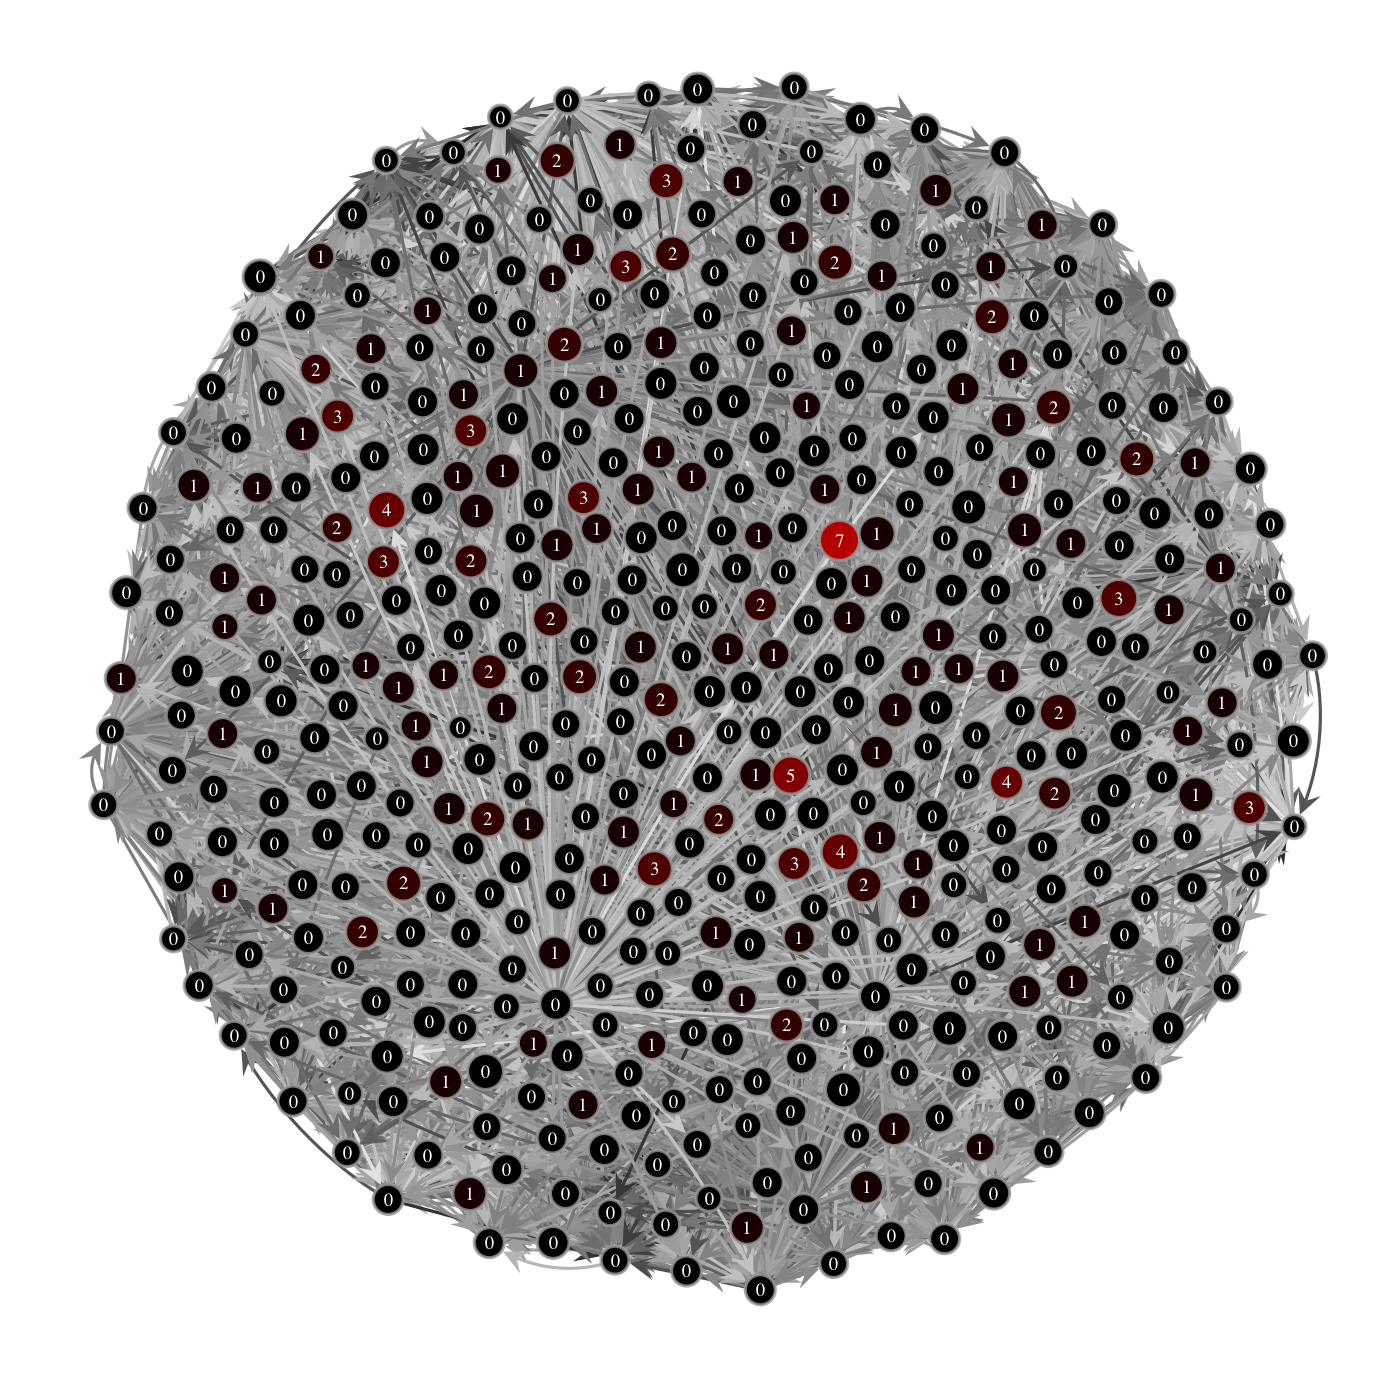
\includegraphics[scale=0.3]{graph_1200_memories.png}
    \caption[Interference accumulation per node of Neuroidal model at 1200 memories]{Interference accumulation per node of Neuroidal model at 1200 memories. \textmd{Neuroidal model (n=500, d=128, w=16, r=40) at 1200 memories. Node value indicates number of interferences that occured at each node.}}
    \label{fig:sub1}
\end{figure}

\begin{figure}%[h]
    \centering
    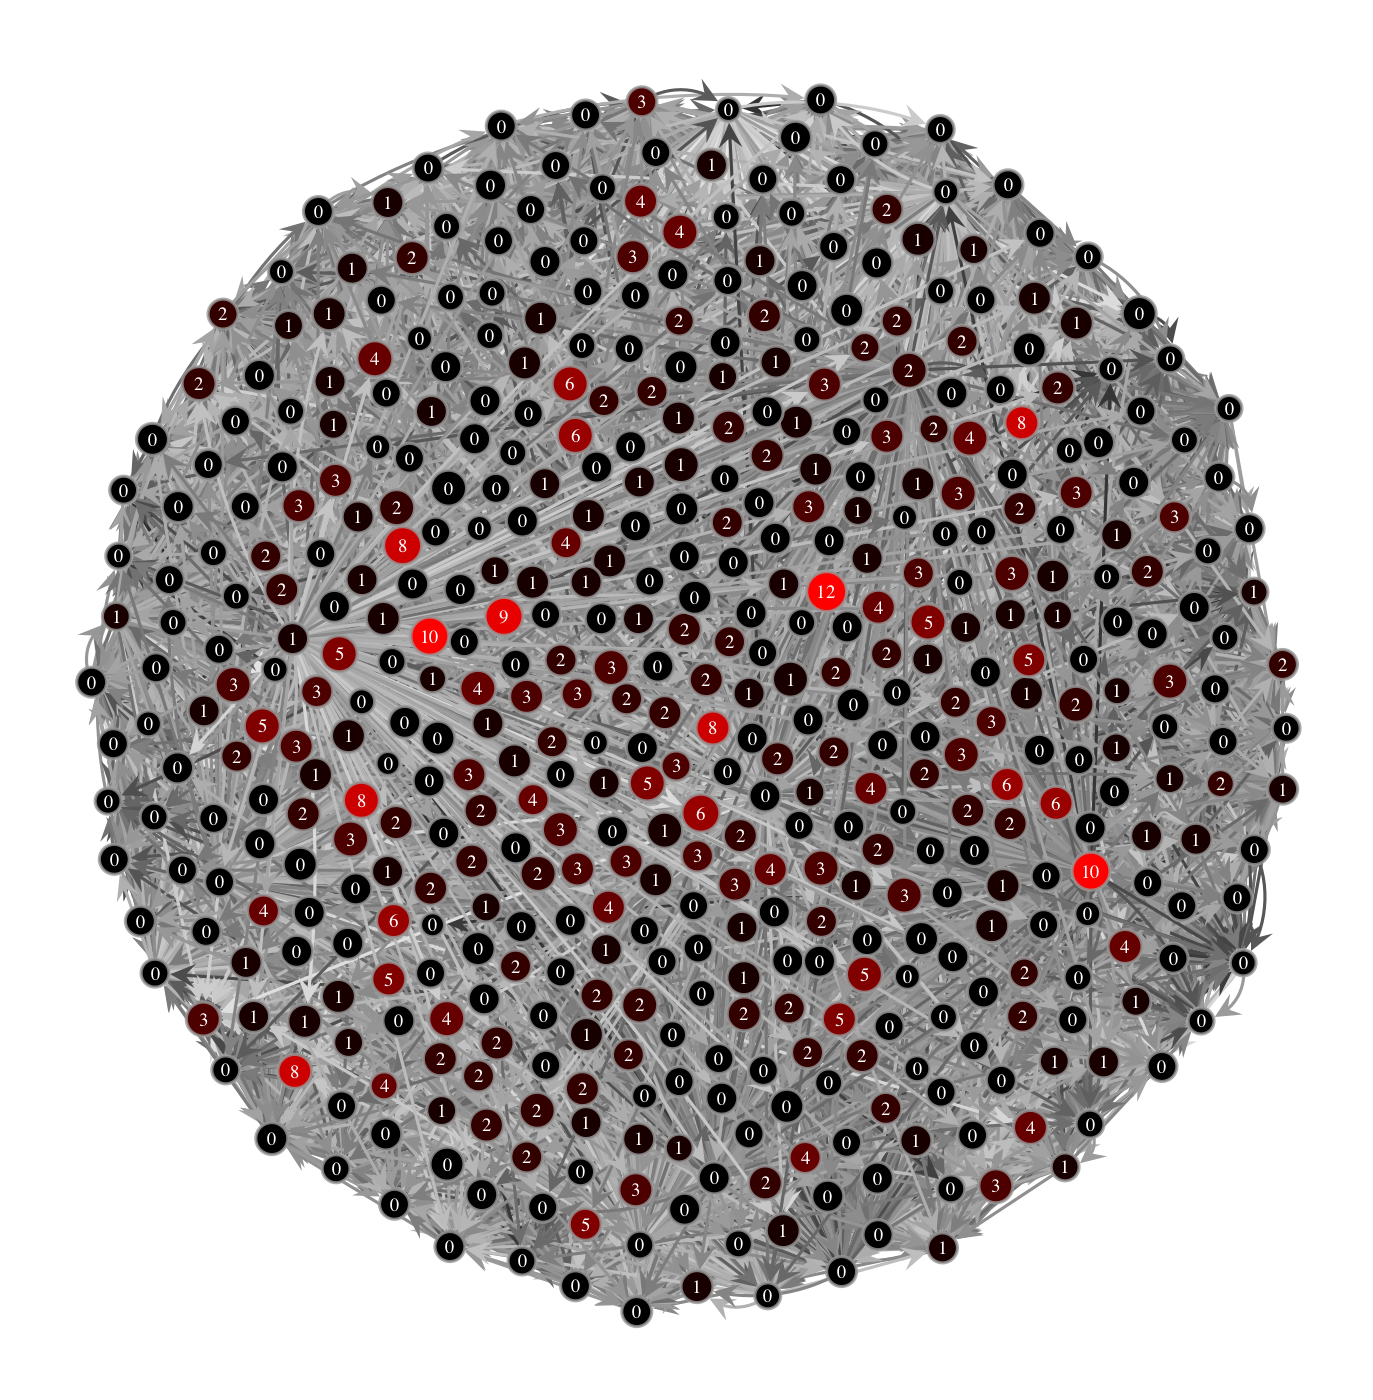
\includegraphics[scale=0.3]{graph_1400_memories.png}
    \caption[Interference accumulation per node of Neuroidal model at 1400 memories]{Interference accumulation per node of Neuroidal model at 1400 memories. \textmd{Neuroidal model (n=500, d=128, w=16, r=40) at 1400 memories. Node value indicates number of interferences that occured at each node.}}
    \label{fig:sub2}
\end{figure}

\begin{figure}%[h]
    \centering
    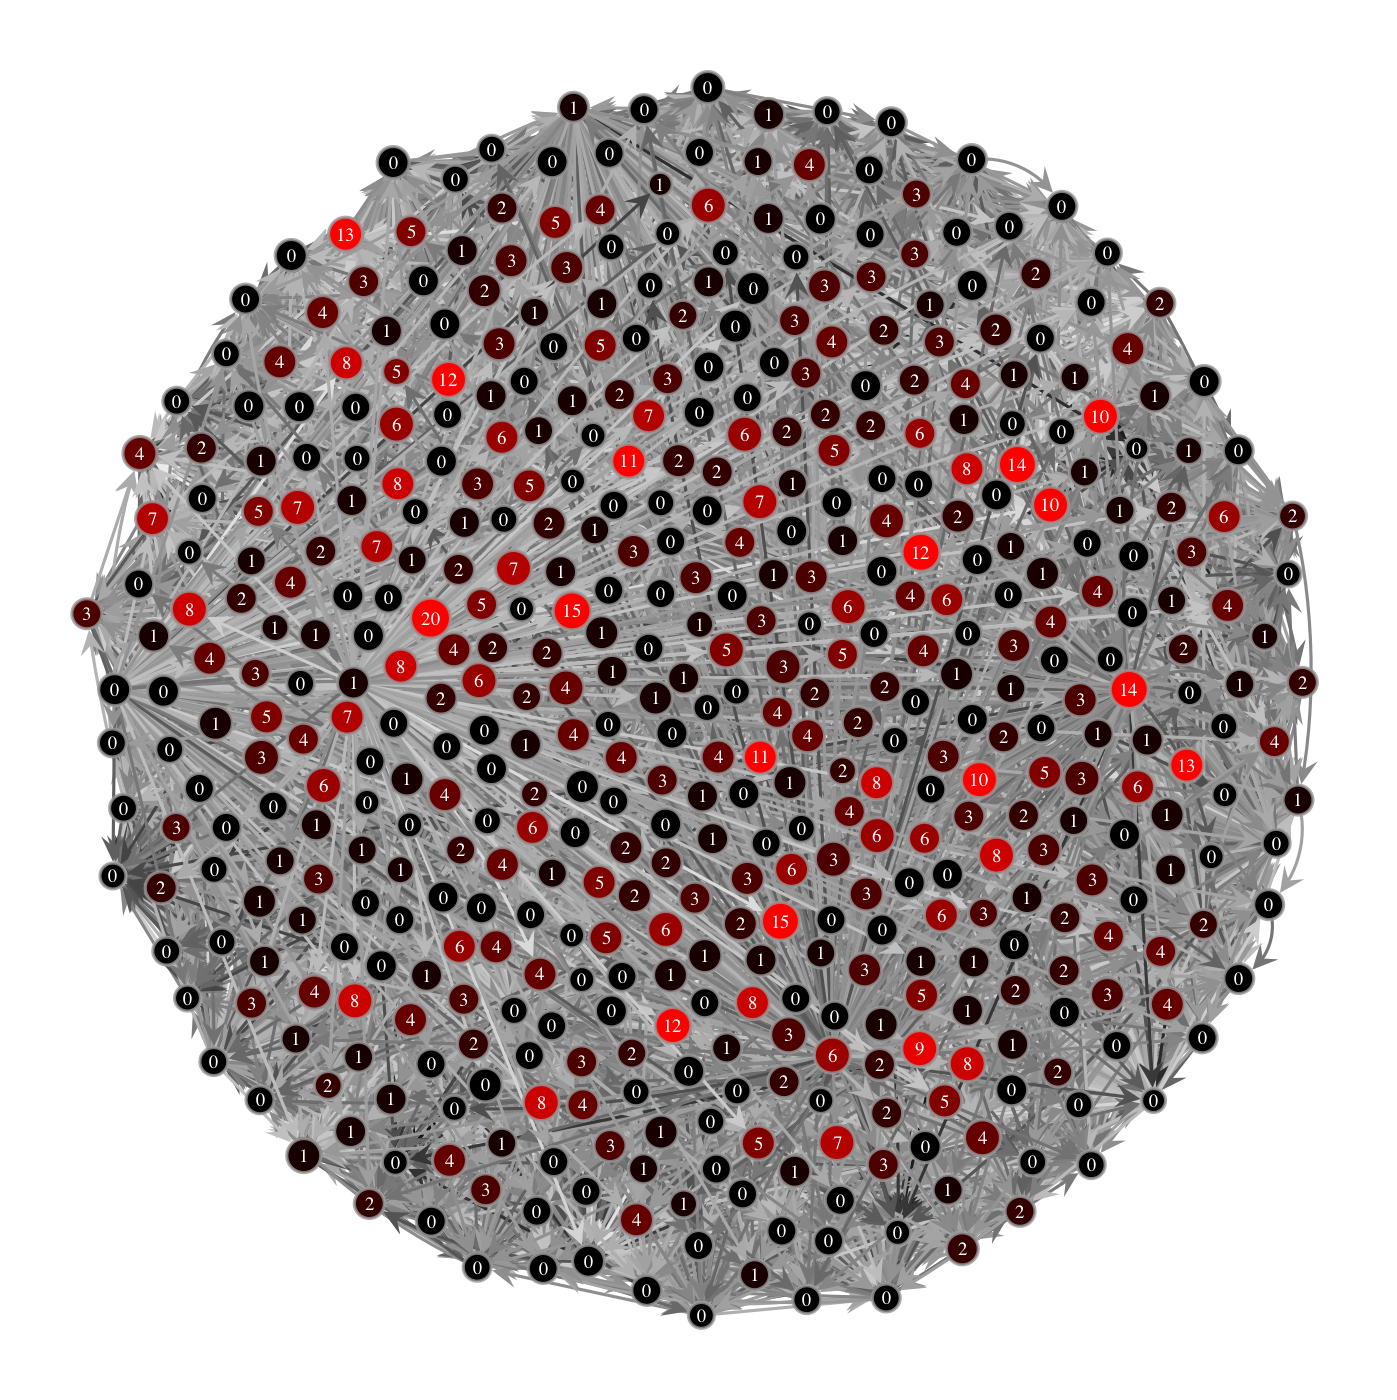
\includegraphics[scale=0.3]{graph_1600_memories.png}
    \caption[Interference accumulation per node of Neuroidal model at 1600 memories]{Interference accumulation per node of Neuroidal model at 1600 memories. \textmd{Neuroidal model (n=500, d=128, w=16, r=40) at 1600 memories. Node value indicates number of interferences that occured at each node.}}
    \label{fig:sub3}
\end{figure}

\begin{figure}%[h]
    \centering
    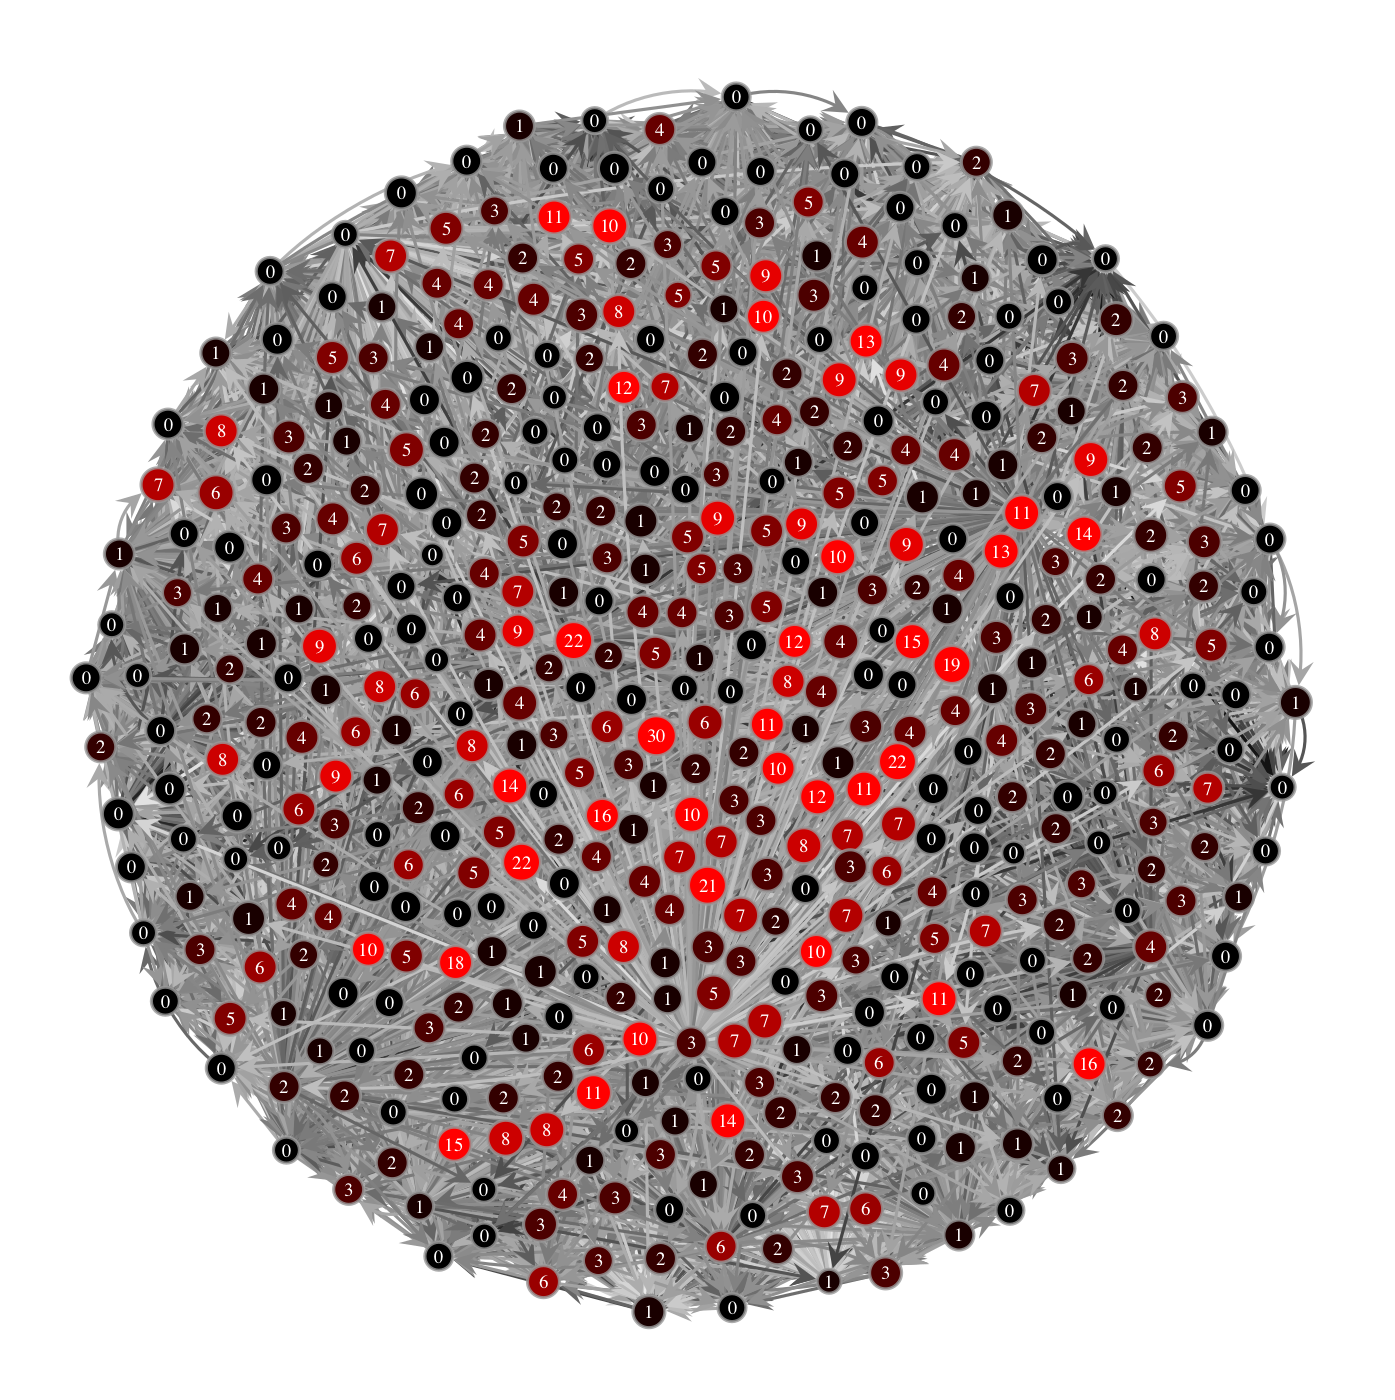
\includegraphics[scale=0.3]{graph_final_memories.png}
    \caption[Interference accumulation per node of Neuroidal model at capacity]{Interference accumulation per node of Neuroidal model at capacity. \textmd{Neuroidal model (n=500, d=128, w=16, r=40) at capacity (1800 memories). Node value indicates number of interferences that occured at each node.}}
    \label{fig:sub4}
\end{figure}

\begin{figure}%[h]
    \centering
    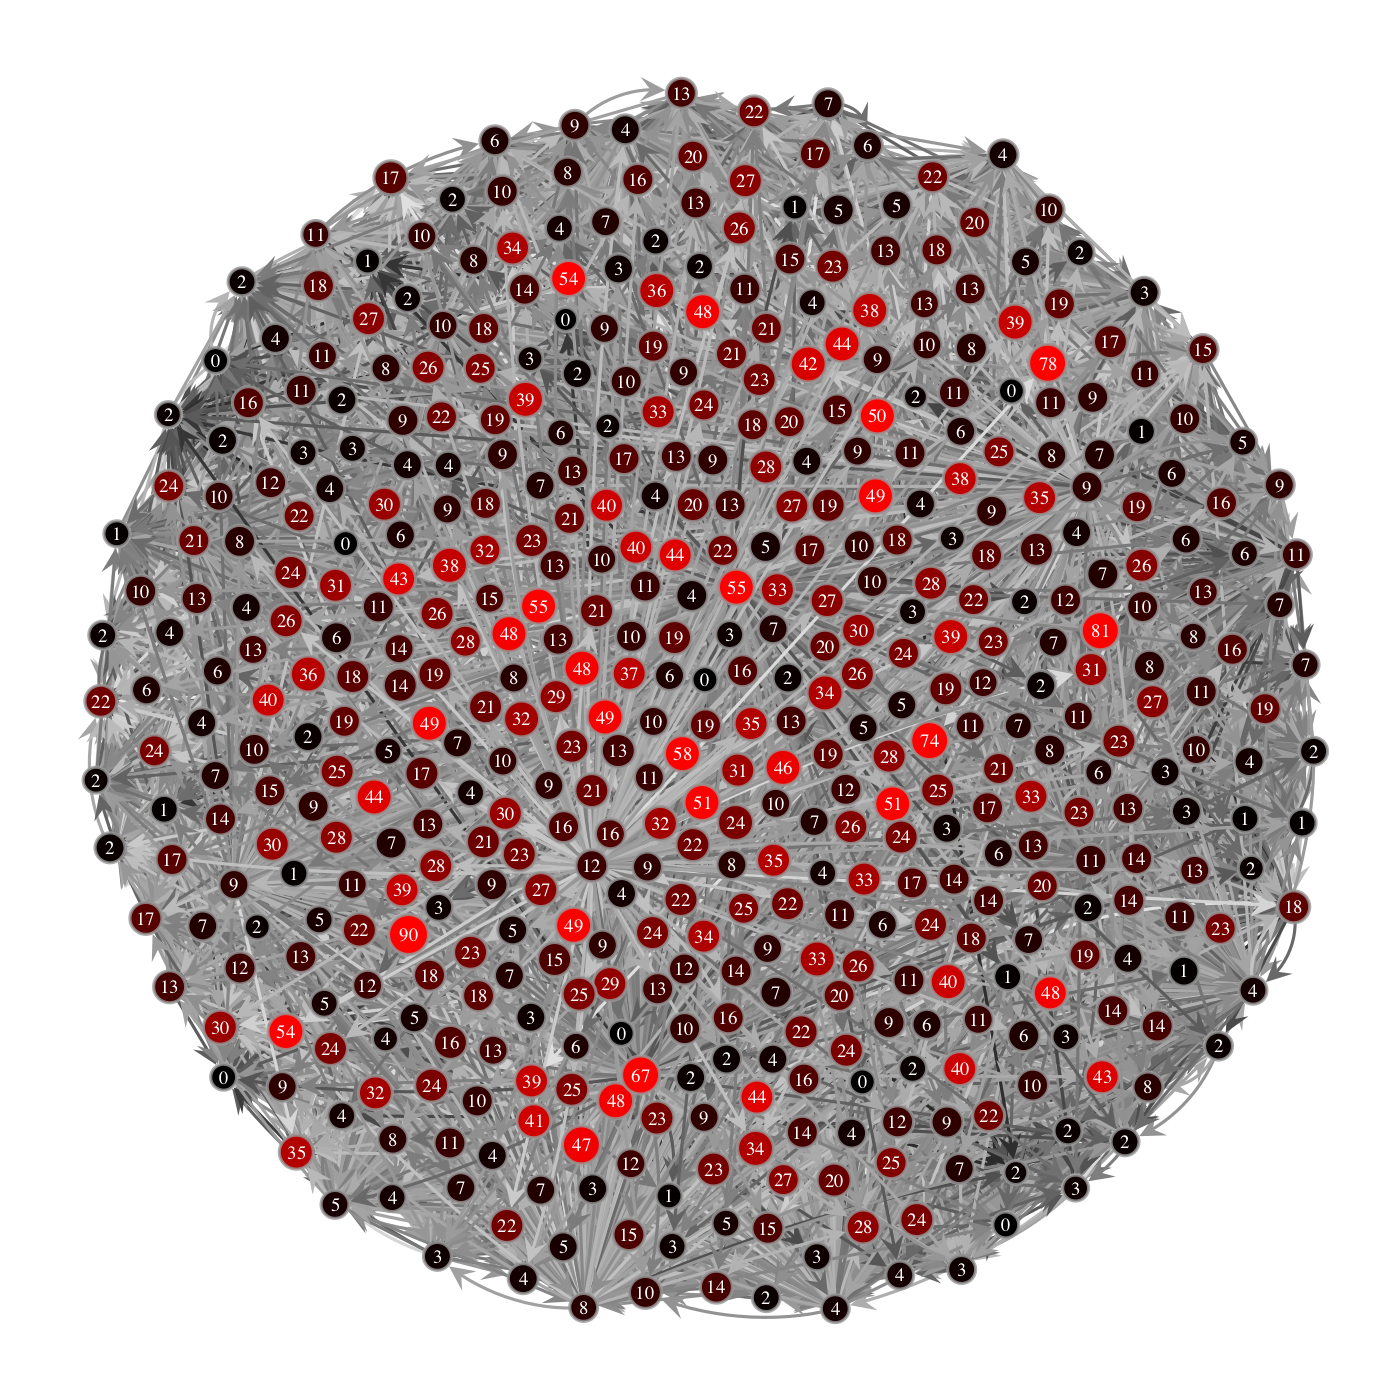
\includegraphics[scale=0.3]{graph_1200_n_memories.png}
    \caption[Memory membership per node of Neuroidal model at 1200 memories]{Memory membership per node of Neuroidal model at 1200 memories. \textmd{Neuroidal model (n=500, d=128, w=16, r=40) at 1200 memories. Node value indicates memory membership of the node.}}
    \label{fig:subn1}
\end{figure}

\begin{figure}%[h]
    \centering
    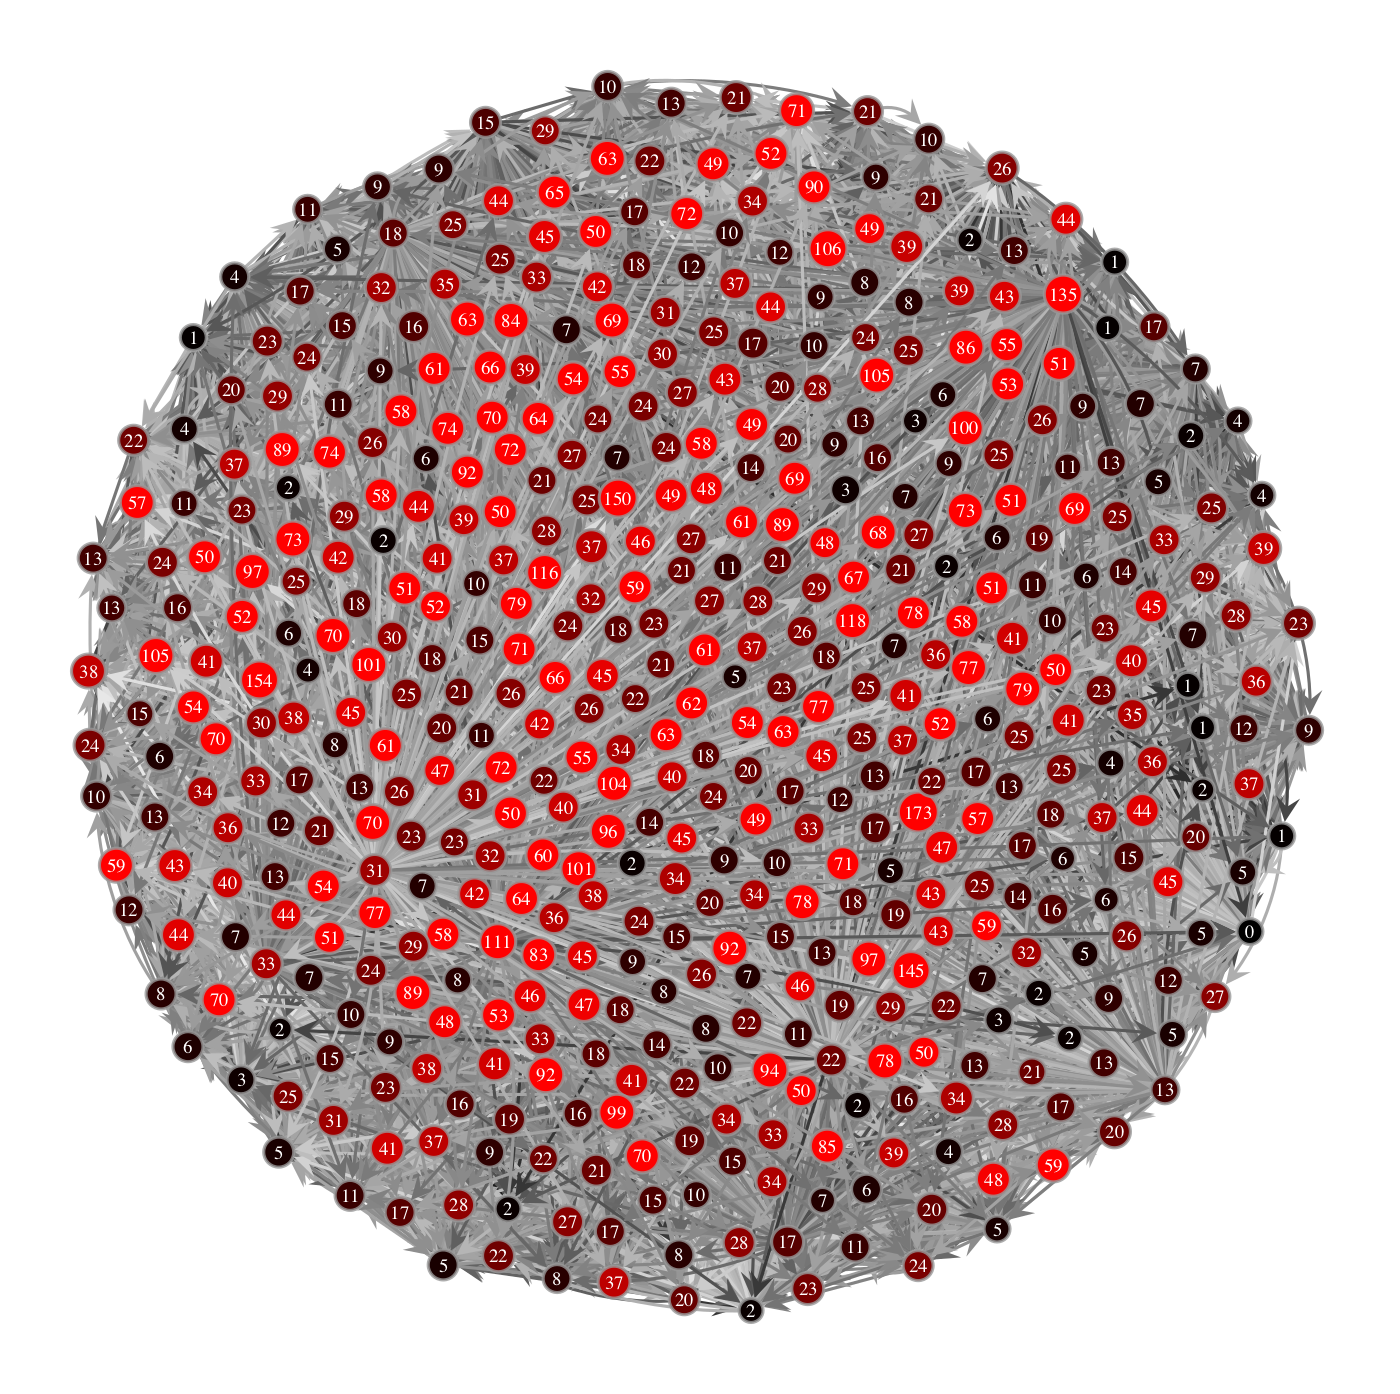
\includegraphics[scale=0.3]{graph_1400_n_memories.png}
    \caption[Memory membership per node of Neuroidal model at 1400 memories]{Memory membership per node of Neuroidal model at 1400 memories. \textmd{Neuroidal model (n=500, d=128, w=16, r=40) at 1400 memories. Node value indicates memory membership of the node.}}
    \label{fig:subn2}
\end{figure}

\begin{figure}%[h]
    \centering
    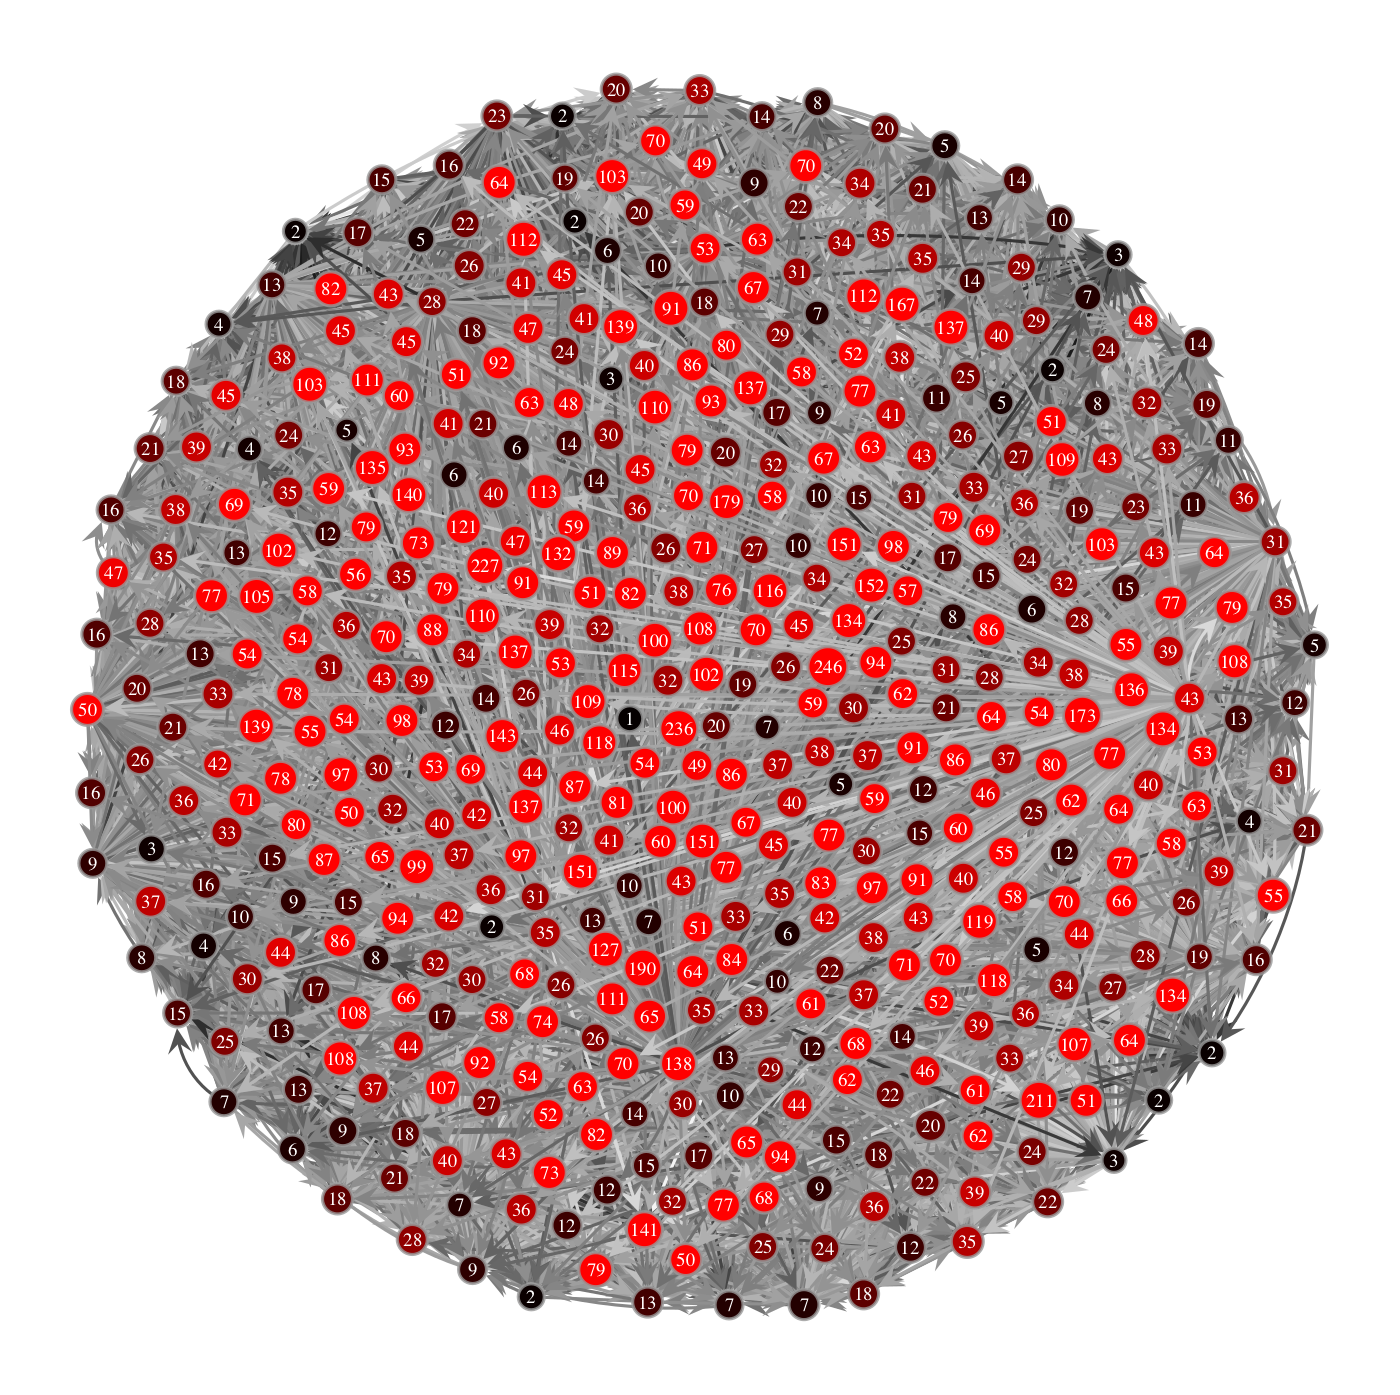
\includegraphics[scale=0.3]{graph_1600_n_memories.png}
    \caption[Memory membership per node of Neuroidal model at 1600 memories]{Memory membership per node of Neuroidal model at 1600 memories. \textmd{Neuroidal model (n=500, d=128, w=16, r=40) at 1600 memories. Node value indicates memory membership of the node.}}
    \label{fig:subn3}
\end{figure}

\begin{figure}%[h]
    \centering
    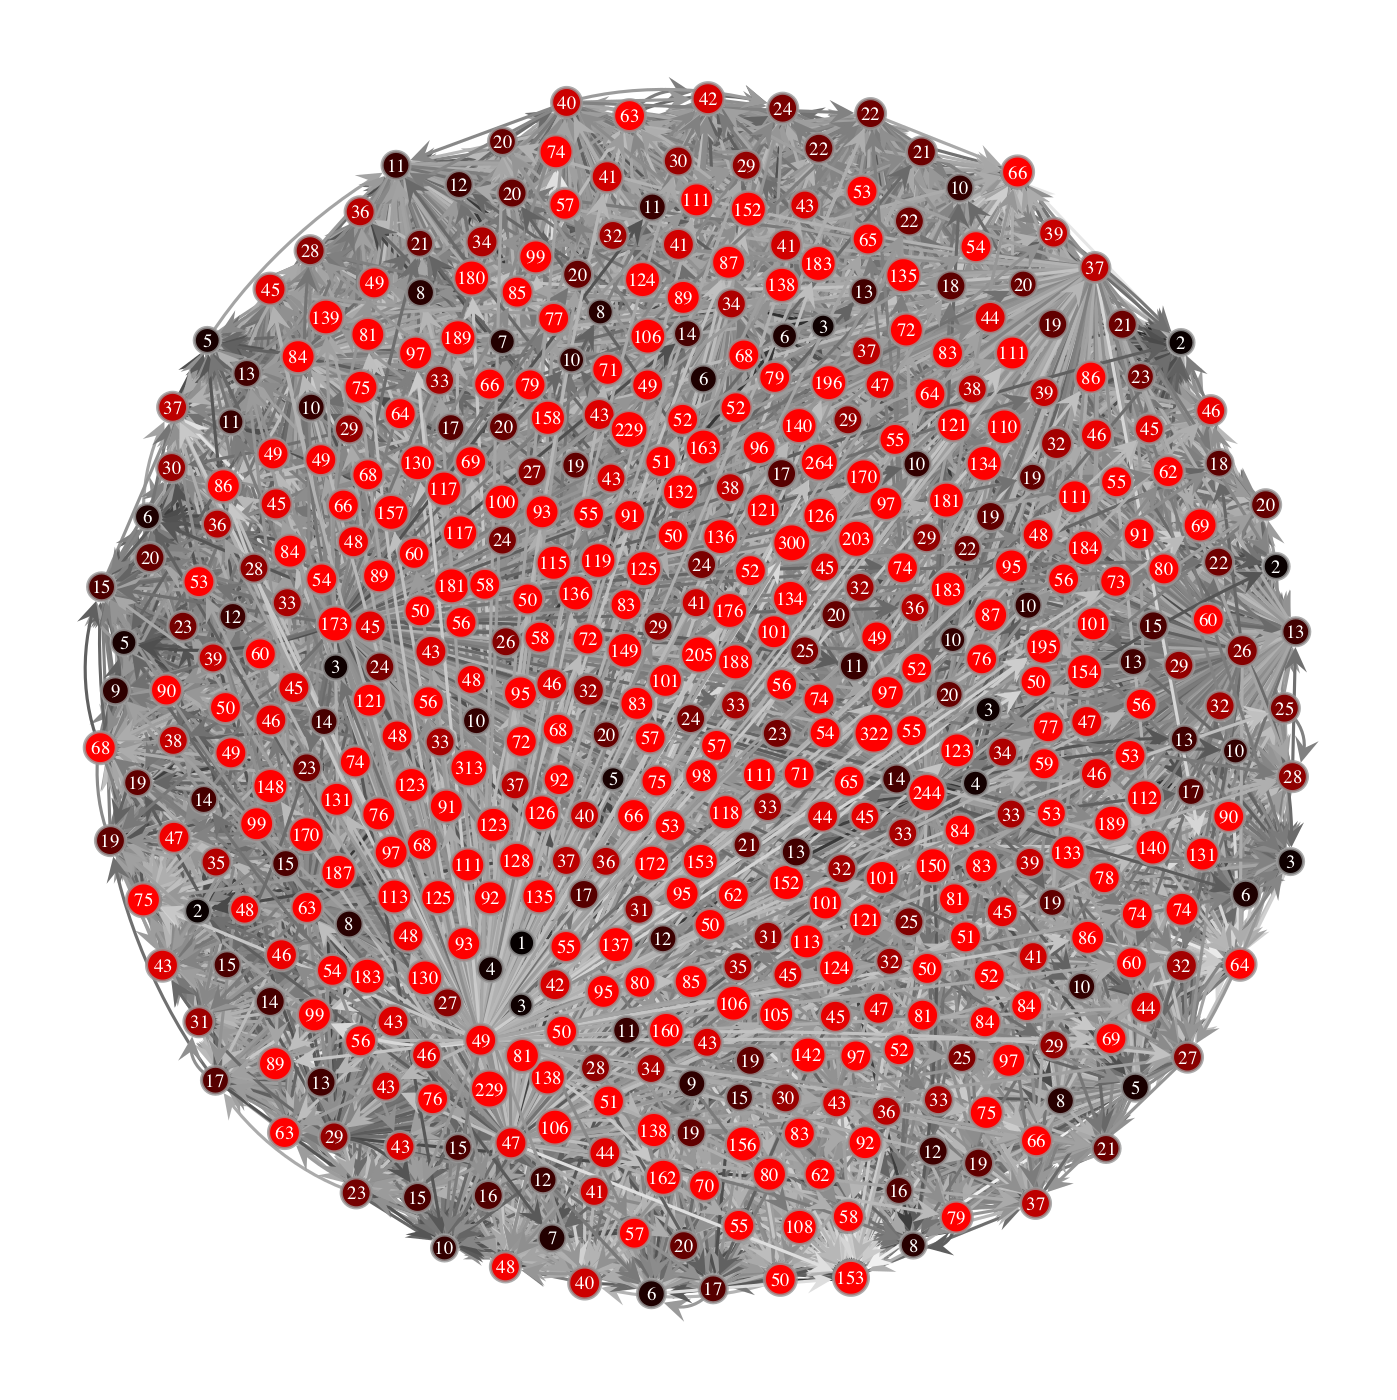
\includegraphics[scale=0.3]{graph_final_n_memories.png}
    \caption[Memory membership per node of Neuroidal model at capacity]{Memory membership per node of Neuroidal model at capacity. \textmd{Neuroidal model (n=500, d=128, w=16, r=40) at capacity (1800 memories). Node value indicates memory membership of the node}}
    \label{fig:subn4}
\end{figure}

Figures \ref{fig:sub1} through \ref{fig:sub4} and \ref{fig:subn1} through \ref{fig:subn4} show the progression of the system from 1200 memories till the system reaches capacity with the value inside the node indicating the number of interferences that occured at that node and the number of memories the node belongs to respectively. The relative size of the node indicates the indegree of the node.  We observe that the interference is not uniformly distributed accross the nodes. And as we observe the pattern of evolution, we see that certain nodes end up with a lot of interference while many have negligible amount of interference. We also note that nodes that have already accumulated some interference have a higher chance of being a center of interference again. Practically, this indicates that some nodes are just innately more prone to interference than other nodes due to the initial edge layout. This is in constrast to our theory which assumes that the nodes are equal at the start and throughout the life of the system. We believe this is the primary factor that will need to be accounted for in attempts to update the theory and in particular, lemma \ref{lemma:k-int-prob} to be compatible with JOIN. We believe this is really challenging and leave it as future work. 

We can also observe from the figures that the number of memories a node is part does not seem to have any correlation to the number of interferences at that node and therefore is not a good indicator of future interference at that node and cannot be used as a heuristic to update our estimate. There does seem to be some correlation between the in-degree and the interference and could provide intuition regarding updating lemma \ref{lemma:k-int-prob}. As such, we feel analyzing the in-degree distribution will be key to finding the capacity for JOIN. 













\chapter{Conclusion}

Inspired by advances in modern computational neuroscience and growing interest in the capacity of the brain, we rigorously defined and studied the notion of ``capacity'' and ``interference'' in a set both theoretically and emprically. We also provided ideas to extend these results to more structured objects like graphs with more advanced algorithms for adding subobjects to the universe.

\section{Future work}

Here we discuss some potential future work building off this study:

\begin{itemize}
    \item Adapt lemma \ref{lemma:k-int-prob} to find the expected interference in the case of other memory creation algorithms like \begin{itemize}
        \item JOIN: This we believe will be the most challenging step as it involves deriving an estimate for the capacity based on the indegree distribution that is non-uniform throughout the graph and also over time. 
        \item Project: We believe that once we have an estimate for JOIN, it will be very easy to find an estimate for Project as these are very similar operations however with slightly different goals. The main thing to note here wil be that assemblies are more densely connected than arbsets and that will the key here. 
        \item Merge: We feel an estimate for merge would be very similar to those of JOIN and Project as it is essentially an amalgation of the two. 
        \item Sequence Project: A analysis of the capacity of Sequence Project will be very interesting as it is the only algorithm we discussed that creates more than a single memory. We are excited to see how this will affect the analysis as well as final estimate. 
    \end{itemize}
    We believe each one of these will provide considerable challenges due to their complex nature \cite{dabagia2023computation, papadimitriou2020brain,valiant2005memorization}. The rest of the theorems will follow similarly to be able to find the capacity of the model and the final expression should have the same general structure. We also think the estimates will follow similar trends against the number of neurons and number of memories. 
    \item Instead of bounding the subset sizes, assume the subset sizes are drawn from a distribution with a given mean $r$ and find the expected subset capacity. This will involve finding the expectation of the hypergeometric PMF as a function of two random variables. 
\end{itemize}

\section{Closing thoughts}

The study of capacity with regards to interference is really important as computational models of the brain need to keep the number of misfires low to be able to accumulate memories for a long period of time as well as maintain a high quality of retrieval.  We believe this study will inspire more computational neuroscientists to tackle the intriguing question of capacity in contemporary models as well as upcoming models that will further demistify the human brain. 



\nocite{*}
\bibliography{bibliography}

% Indents Appendix in Table of Contents
\makeatletter
\addtocontents{toc}{\let\protect\l@chapter\protect\l@section}
\makeatother

% Hack to make Appendices to appear in Table of Contents
\addtocontents{toc}{%
   \noindent APPENDICES
}
\begin{appendices}
\input{appendix-outline}
\end{appendices}

\end{document}
